\chapter{Driven cavity problem}

\begin{figure}[h]
	\centering
	\begin{subfigure}{0.5\textwidth}
		\resizebox{1.4\textwidth}{!}{% GNUPLOT: LaTeX picture with Postscript
\begingroup
  \makeatletter
  \providecommand\color[2][]{%
    \GenericError{(gnuplot) \space\space\space\@spaces}{%
      Package color not loaded in conjunction with
      terminal option `colourtext'%
    }{See the gnuplot documentation for explanation.%
    }{Either use 'blacktext' in gnuplot or load the package
      color.sty in LaTeX.}%
    \renewcommand\color[2][]{}%
  }%
  \providecommand\includegraphics[2][]{%
    \GenericError{(gnuplot) \space\space\space\@spaces}{%
      Package graphicx or graphics not loaded%
    }{See the gnuplot documentation for explanation.%
    }{The gnuplot epslatex terminal needs graphicx.sty or graphics.sty.}%
    \renewcommand\includegraphics[2][]{}%
  }%
  \providecommand\rotatebox[2]{#2}%
  \@ifundefined{ifGPcolor}{%
    \newif\ifGPcolor
    \GPcolortrue
  }{}%
  \@ifundefined{ifGPblacktext}{%
    \newif\ifGPblacktext
    \GPblacktexttrue
  }{}%
  % define a \g@addto@macro without @ in the name:
  \let\gplgaddtomacro\g@addto@macro
  % define empty templates for all commands taking text:
  \gdef\gplbacktext{}%
  \gdef\gplfronttext{}%
  \makeatother
  \ifGPblacktext
    % no textcolor at all
    \def\colorrgb#1{}%
    \def\colorgray#1{}%
  \else
    % gray or color?
    \ifGPcolor
      \def\colorrgb#1{\color[rgb]{#1}}%
      \def\colorgray#1{\color[gray]{#1}}%
      \expandafter\def\csname LTw\endcsname{\color{white}}%
      \expandafter\def\csname LTb\endcsname{\color{black}}%
      \expandafter\def\csname LTa\endcsname{\color{black}}%
      \expandafter\def\csname LT0\endcsname{\color[rgb]{1,0,0}}%
      \expandafter\def\csname LT1\endcsname{\color[rgb]{0,1,0}}%
      \expandafter\def\csname LT2\endcsname{\color[rgb]{0,0,1}}%
      \expandafter\def\csname LT3\endcsname{\color[rgb]{1,0,1}}%
      \expandafter\def\csname LT4\endcsname{\color[rgb]{0,1,1}}%
      \expandafter\def\csname LT5\endcsname{\color[rgb]{1,1,0}}%
      \expandafter\def\csname LT6\endcsname{\color[rgb]{0,0,0}}%
      \expandafter\def\csname LT7\endcsname{\color[rgb]{1,0.3,0}}%
      \expandafter\def\csname LT8\endcsname{\color[rgb]{0.5,0.5,0.5}}%
    \else
      % gray
      \def\colorrgb#1{\color{black}}%
      \def\colorgray#1{\color[gray]{#1}}%
      \expandafter\def\csname LTw\endcsname{\color{white}}%
      \expandafter\def\csname LTb\endcsname{\color{black}}%
      \expandafter\def\csname LTa\endcsname{\color{black}}%
      \expandafter\def\csname LT0\endcsname{\color{black}}%
      \expandafter\def\csname LT1\endcsname{\color{black}}%
      \expandafter\def\csname LT2\endcsname{\color{black}}%
      \expandafter\def\csname LT3\endcsname{\color{black}}%
      \expandafter\def\csname LT4\endcsname{\color{black}}%
      \expandafter\def\csname LT5\endcsname{\color{black}}%
      \expandafter\def\csname LT6\endcsname{\color{black}}%
      \expandafter\def\csname LT7\endcsname{\color{black}}%
      \expandafter\def\csname LT8\endcsname{\color{black}}%
    \fi
  \fi
    \setlength{\unitlength}{0.0500bp}%
    \ifx\gptboxheight\undefined%
      \newlength{\gptboxheight}%
      \newlength{\gptboxwidth}%
      \newsavebox{\gptboxtext}%
    \fi%
    \setlength{\fboxrule}{0.5pt}%
    \setlength{\fboxsep}{1pt}%
\begin{picture}(7200.00,5040.00)%
    \gplgaddtomacro\gplbacktext{%
      \csname LTb\endcsname%
      \put(1487,484){\makebox(0,0)[r]{\strut{}$0$}}%
      \put(1487,1342){\makebox(0,0)[r]{\strut{}$0.2$}}%
      \put(1487,2200){\makebox(0,0)[r]{\strut{}$0.4$}}%
      \put(1487,3059){\makebox(0,0)[r]{\strut{}$0.6$}}%
      \put(1487,3917){\makebox(0,0)[r]{\strut{}$0.8$}}%
      \put(1487,4775){\makebox(0,0)[r]{\strut{}$1$}}%
      \put(1619,264){\makebox(0,0){\strut{}$-0.4$}}%
      \put(2232,264){\makebox(0,0){\strut{}$-0.2$}}%
      \put(2845,264){\makebox(0,0){\strut{}$0$}}%
      \put(3458,264){\makebox(0,0){\strut{}$0.2$}}%
      \put(4071,264){\makebox(0,0){\strut{}$0.4$}}%
      \put(4684,264){\makebox(0,0){\strut{}$0.6$}}%
      \put(5297,264){\makebox(0,0){\strut{}$0.8$}}%
      \put(5910,264){\makebox(0,0){\strut{}$1$}}%
    }%
    \gplgaddtomacro\gplfronttext{%
      \csname LTb\endcsname%
      \put(1245,4829){\makebox(0,0){\strut{}y}}%
      \put(3764,154){\makebox(0,0){\strut{}u}}%
      \csname LTb\endcsname%
      \put(3071,4602){\makebox(0,0)[r]{\strut{}Calculated}}%
      \csname LTb\endcsname%
      \put(3071,4382){\makebox(0,0)[r]{\strut{}Reference}}%
    }%
    \gplbacktext
    \put(0,0){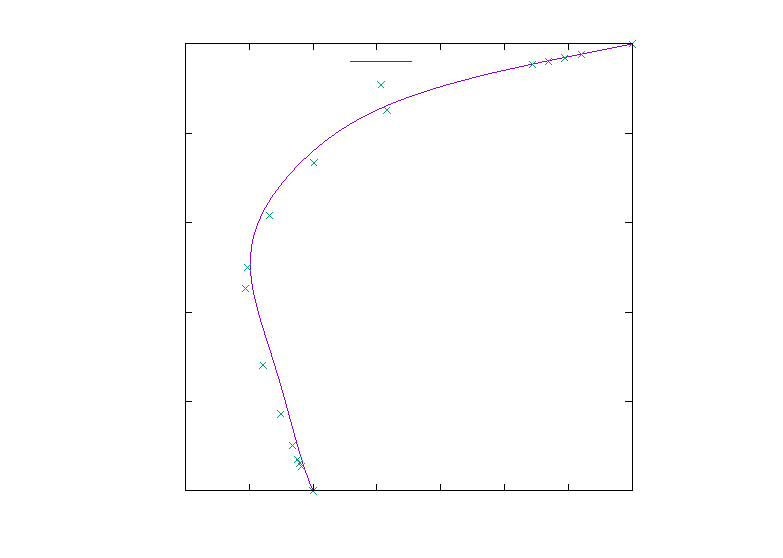
\includegraphics{DrivenCavity/u100}}%
    \gplfronttext
  \end{picture}%
\endgroup
}
		\caption{$Re=100$}
	\end{subfigure}%
	\begin{subfigure}{0.5\textwidth}
		\resizebox{1.4\textwidth}{!}{% GNUPLOT: LaTeX picture with Postscript
\begingroup
  \makeatletter
  \providecommand\color[2][]{%
    \GenericError{(gnuplot) \space\space\space\@spaces}{%
      Package color not loaded in conjunction with
      terminal option `colourtext'%
    }{See the gnuplot documentation for explanation.%
    }{Either use 'blacktext' in gnuplot or load the package
      color.sty in LaTeX.}%
    \renewcommand\color[2][]{}%
  }%
  \providecommand\includegraphics[2][]{%
    \GenericError{(gnuplot) \space\space\space\@spaces}{%
      Package graphicx or graphics not loaded%
    }{See the gnuplot documentation for explanation.%
    }{The gnuplot epslatex terminal needs graphicx.sty or graphics.sty.}%
    \renewcommand\includegraphics[2][]{}%
  }%
  \providecommand\rotatebox[2]{#2}%
  \@ifundefined{ifGPcolor}{%
    \newif\ifGPcolor
    \GPcolortrue
  }{}%
  \@ifundefined{ifGPblacktext}{%
    \newif\ifGPblacktext
    \GPblacktexttrue
  }{}%
  % define a \g@addto@macro without @ in the name:
  \let\gplgaddtomacro\g@addto@macro
  % define empty templates for all commands taking text:
  \gdef\gplbacktext{}%
  \gdef\gplfronttext{}%
  \makeatother
  \ifGPblacktext
    % no textcolor at all
    \def\colorrgb#1{}%
    \def\colorgray#1{}%
  \else
    % gray or color?
    \ifGPcolor
      \def\colorrgb#1{\color[rgb]{#1}}%
      \def\colorgray#1{\color[gray]{#1}}%
      \expandafter\def\csname LTw\endcsname{\color{white}}%
      \expandafter\def\csname LTb\endcsname{\color{black}}%
      \expandafter\def\csname LTa\endcsname{\color{black}}%
      \expandafter\def\csname LT0\endcsname{\color[rgb]{1,0,0}}%
      \expandafter\def\csname LT1\endcsname{\color[rgb]{0,1,0}}%
      \expandafter\def\csname LT2\endcsname{\color[rgb]{0,0,1}}%
      \expandafter\def\csname LT3\endcsname{\color[rgb]{1,0,1}}%
      \expandafter\def\csname LT4\endcsname{\color[rgb]{0,1,1}}%
      \expandafter\def\csname LT5\endcsname{\color[rgb]{1,1,0}}%
      \expandafter\def\csname LT6\endcsname{\color[rgb]{0,0,0}}%
      \expandafter\def\csname LT7\endcsname{\color[rgb]{1,0.3,0}}%
      \expandafter\def\csname LT8\endcsname{\color[rgb]{0.5,0.5,0.5}}%
    \else
      % gray
      \def\colorrgb#1{\color{black}}%
      \def\colorgray#1{\color[gray]{#1}}%
      \expandafter\def\csname LTw\endcsname{\color{white}}%
      \expandafter\def\csname LTb\endcsname{\color{black}}%
      \expandafter\def\csname LTa\endcsname{\color{black}}%
      \expandafter\def\csname LT0\endcsname{\color{black}}%
      \expandafter\def\csname LT1\endcsname{\color{black}}%
      \expandafter\def\csname LT2\endcsname{\color{black}}%
      \expandafter\def\csname LT3\endcsname{\color{black}}%
      \expandafter\def\csname LT4\endcsname{\color{black}}%
      \expandafter\def\csname LT5\endcsname{\color{black}}%
      \expandafter\def\csname LT6\endcsname{\color{black}}%
      \expandafter\def\csname LT7\endcsname{\color{black}}%
      \expandafter\def\csname LT8\endcsname{\color{black}}%
    \fi
  \fi
    \setlength{\unitlength}{0.0500bp}%
    \ifx\gptboxheight\undefined%
      \newlength{\gptboxheight}%
      \newlength{\gptboxwidth}%
      \newsavebox{\gptboxtext}%
    \fi%
    \setlength{\fboxrule}{0.5pt}%
    \setlength{\fboxsep}{1pt}%
\begin{picture}(7200.00,5040.00)%
    \gplgaddtomacro\gplbacktext{%
      \csname LTb\endcsname%
      \put(1487,484){\makebox(0,0)[r]{\strut{}$0$}}%
      \put(1487,1342){\makebox(0,0)[r]{\strut{}$0.2$}}%
      \put(1487,2200){\makebox(0,0)[r]{\strut{}$0.4$}}%
      \put(1487,3059){\makebox(0,0)[r]{\strut{}$0.6$}}%
      \put(1487,3917){\makebox(0,0)[r]{\strut{}$0.8$}}%
      \put(1487,4775){\makebox(0,0)[r]{\strut{}$1$}}%
      \put(1619,264){\makebox(0,0){\strut{}$-0.4$}}%
      \put(2232,264){\makebox(0,0){\strut{}$-0.2$}}%
      \put(2845,264){\makebox(0,0){\strut{}$0$}}%
      \put(3458,264){\makebox(0,0){\strut{}$0.2$}}%
      \put(4071,264){\makebox(0,0){\strut{}$0.4$}}%
      \put(4684,264){\makebox(0,0){\strut{}$0.6$}}%
      \put(5297,264){\makebox(0,0){\strut{}$0.8$}}%
      \put(5910,264){\makebox(0,0){\strut{}$1$}}%
    }%
    \gplgaddtomacro\gplfronttext{%
      \csname LTb\endcsname%
      \put(1245,4829){\makebox(0,0){\strut{}y}}%
      \put(3764,154){\makebox(0,0){\strut{}u}}%
      \csname LTb\endcsname%
      \put(3071,4602){\makebox(0,0)[r]{\strut{}Calculated}}%
      \csname LTb\endcsname%
      \put(3071,4382){\makebox(0,0)[r]{\strut{}Reference}}%
    }%
    \gplbacktext
    \put(0,0){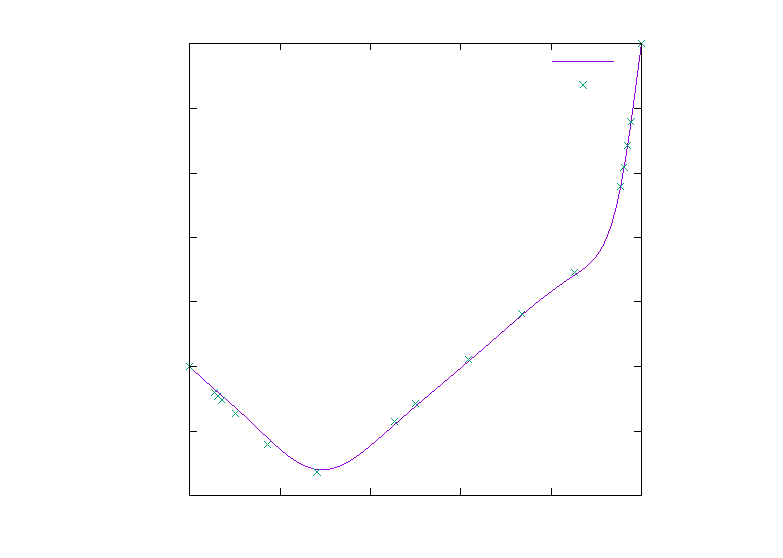
\includegraphics{DrivenCavity/u400}}%
    \gplfronttext
  \end{picture}%
\endgroup
}
		\caption{$Re=400$}
	\end{subfigure}
	\begin{subfigure}{0.5\textwidth}
		\resizebox{1.4\textwidth}{!}{% GNUPLOT: LaTeX picture with Postscript
\begingroup
  \makeatletter
  \providecommand\color[2][]{%
    \GenericError{(gnuplot) \space\space\space\@spaces}{%
      Package color not loaded in conjunction with
      terminal option `colourtext'%
    }{See the gnuplot documentation for explanation.%
    }{Either use 'blacktext' in gnuplot or load the package
      color.sty in LaTeX.}%
    \renewcommand\color[2][]{}%
  }%
  \providecommand\includegraphics[2][]{%
    \GenericError{(gnuplot) \space\space\space\@spaces}{%
      Package graphicx or graphics not loaded%
    }{See the gnuplot documentation for explanation.%
    }{The gnuplot epslatex terminal needs graphicx.sty or graphics.sty.}%
    \renewcommand\includegraphics[2][]{}%
  }%
  \providecommand\rotatebox[2]{#2}%
  \@ifundefined{ifGPcolor}{%
    \newif\ifGPcolor
    \GPcolortrue
  }{}%
  \@ifundefined{ifGPblacktext}{%
    \newif\ifGPblacktext
    \GPblacktexttrue
  }{}%
  % define a \g@addto@macro without @ in the name:
  \let\gplgaddtomacro\g@addto@macro
  % define empty templates for all commands taking text:
  \gdef\gplbacktext{}%
  \gdef\gplfronttext{}%
  \makeatother
  \ifGPblacktext
    % no textcolor at all
    \def\colorrgb#1{}%
    \def\colorgray#1{}%
  \else
    % gray or color?
    \ifGPcolor
      \def\colorrgb#1{\color[rgb]{#1}}%
      \def\colorgray#1{\color[gray]{#1}}%
      \expandafter\def\csname LTw\endcsname{\color{white}}%
      \expandafter\def\csname LTb\endcsname{\color{black}}%
      \expandafter\def\csname LTa\endcsname{\color{black}}%
      \expandafter\def\csname LT0\endcsname{\color[rgb]{1,0,0}}%
      \expandafter\def\csname LT1\endcsname{\color[rgb]{0,1,0}}%
      \expandafter\def\csname LT2\endcsname{\color[rgb]{0,0,1}}%
      \expandafter\def\csname LT3\endcsname{\color[rgb]{1,0,1}}%
      \expandafter\def\csname LT4\endcsname{\color[rgb]{0,1,1}}%
      \expandafter\def\csname LT5\endcsname{\color[rgb]{1,1,0}}%
      \expandafter\def\csname LT6\endcsname{\color[rgb]{0,0,0}}%
      \expandafter\def\csname LT7\endcsname{\color[rgb]{1,0.3,0}}%
      \expandafter\def\csname LT8\endcsname{\color[rgb]{0.5,0.5,0.5}}%
    \else
      % gray
      \def\colorrgb#1{\color{black}}%
      \def\colorgray#1{\color[gray]{#1}}%
      \expandafter\def\csname LTw\endcsname{\color{white}}%
      \expandafter\def\csname LTb\endcsname{\color{black}}%
      \expandafter\def\csname LTa\endcsname{\color{black}}%
      \expandafter\def\csname LT0\endcsname{\color{black}}%
      \expandafter\def\csname LT1\endcsname{\color{black}}%
      \expandafter\def\csname LT2\endcsname{\color{black}}%
      \expandafter\def\csname LT3\endcsname{\color{black}}%
      \expandafter\def\csname LT4\endcsname{\color{black}}%
      \expandafter\def\csname LT5\endcsname{\color{black}}%
      \expandafter\def\csname LT6\endcsname{\color{black}}%
      \expandafter\def\csname LT7\endcsname{\color{black}}%
      \expandafter\def\csname LT8\endcsname{\color{black}}%
    \fi
  \fi
    \setlength{\unitlength}{0.0500bp}%
    \ifx\gptboxheight\undefined%
      \newlength{\gptboxheight}%
      \newlength{\gptboxwidth}%
      \newsavebox{\gptboxtext}%
    \fi%
    \setlength{\fboxrule}{0.5pt}%
    \setlength{\fboxsep}{1pt}%
\begin{picture}(7200.00,5040.00)%
    \gplgaddtomacro\gplbacktext{%
      \csname LTb\endcsname%
      \put(1531,440){\makebox(0,0)[r]{\strut{}$-0.4$}}%
      \put(1531,1059){\makebox(0,0)[r]{\strut{}$-0.2$}}%
      \put(1531,1679){\makebox(0,0)[r]{\strut{}$0$}}%
      \put(1531,2298){\makebox(0,0)[r]{\strut{}$0.2$}}%
      \put(1531,2917){\makebox(0,0)[r]{\strut{}$0.4$}}%
      \put(1531,3536){\makebox(0,0)[r]{\strut{}$0.6$}}%
      \put(1531,4156){\makebox(0,0)[r]{\strut{}$0.8$}}%
      \put(1531,4775){\makebox(0,0)[r]{\strut{}$1$}}%
      \put(1663,220){\makebox(0,0){\strut{}$0$}}%
      \put(2530,220){\makebox(0,0){\strut{}$0.2$}}%
      \put(3397,220){\makebox(0,0){\strut{}$0.4$}}%
      \put(4264,220){\makebox(0,0){\strut{}$0.6$}}%
      \put(5131,220){\makebox(0,0){\strut{}$0.8$}}%
      \put(5998,220){\makebox(0,0){\strut{}$1$}}%
    }%
    \gplgaddtomacro\gplfronttext{%
      \csname LTb\endcsname%
      \put(5011,4602){\makebox(0,0)[r]{\strut{}Calculated}}%
      \csname LTb\endcsname%
      \put(5011,4382){\makebox(0,0)[r]{\strut{}Reference}}%
    }%
    \gplbacktext
    \put(0,0){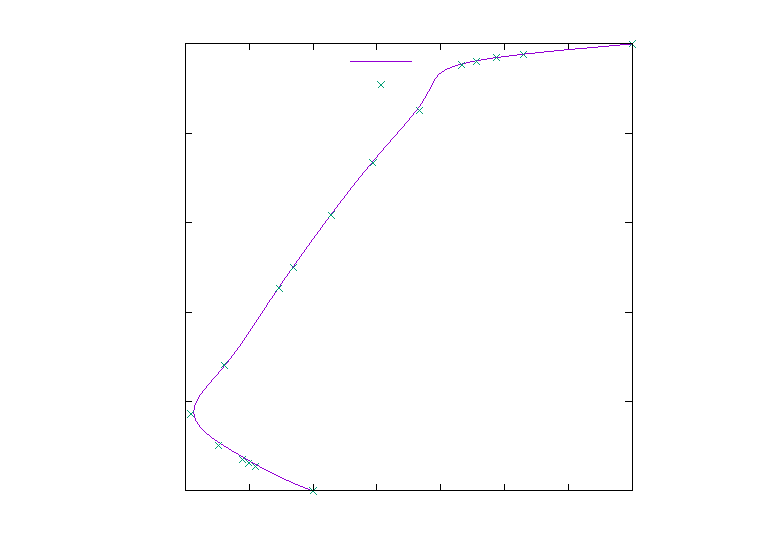
\includegraphics{u1000}}%
    \gplfronttext
  \end{picture}%
\endgroup
}
		\caption{$Re=1000$}
	\end{subfigure}%
	\begin{subfigure}{0.5\textwidth}
		\resizebox{1.4\textwidth}{!}{% GNUPLOT: LaTeX picture with Postscript
\begingroup
  \makeatletter
  \providecommand\color[2][]{%
    \GenericError{(gnuplot) \space\space\space\@spaces}{%
      Package color not loaded in conjunction with
      terminal option `colourtext'%
    }{See the gnuplot documentation for explanation.%
    }{Either use 'blacktext' in gnuplot or load the package
      color.sty in LaTeX.}%
    \renewcommand\color[2][]{}%
  }%
  \providecommand\includegraphics[2][]{%
    \GenericError{(gnuplot) \space\space\space\@spaces}{%
      Package graphicx or graphics not loaded%
    }{See the gnuplot documentation for explanation.%
    }{The gnuplot epslatex terminal needs graphicx.sty or graphics.sty.}%
    \renewcommand\includegraphics[2][]{}%
  }%
  \providecommand\rotatebox[2]{#2}%
  \@ifundefined{ifGPcolor}{%
    \newif\ifGPcolor
    \GPcolortrue
  }{}%
  \@ifundefined{ifGPblacktext}{%
    \newif\ifGPblacktext
    \GPblacktexttrue
  }{}%
  % define a \g@addto@macro without @ in the name:
  \let\gplgaddtomacro\g@addto@macro
  % define empty templates for all commands taking text:
  \gdef\gplbacktext{}%
  \gdef\gplfronttext{}%
  \makeatother
  \ifGPblacktext
    % no textcolor at all
    \def\colorrgb#1{}%
    \def\colorgray#1{}%
  \else
    % gray or color?
    \ifGPcolor
      \def\colorrgb#1{\color[rgb]{#1}}%
      \def\colorgray#1{\color[gray]{#1}}%
      \expandafter\def\csname LTw\endcsname{\color{white}}%
      \expandafter\def\csname LTb\endcsname{\color{black}}%
      \expandafter\def\csname LTa\endcsname{\color{black}}%
      \expandafter\def\csname LT0\endcsname{\color[rgb]{1,0,0}}%
      \expandafter\def\csname LT1\endcsname{\color[rgb]{0,1,0}}%
      \expandafter\def\csname LT2\endcsname{\color[rgb]{0,0,1}}%
      \expandafter\def\csname LT3\endcsname{\color[rgb]{1,0,1}}%
      \expandafter\def\csname LT4\endcsname{\color[rgb]{0,1,1}}%
      \expandafter\def\csname LT5\endcsname{\color[rgb]{1,1,0}}%
      \expandafter\def\csname LT6\endcsname{\color[rgb]{0,0,0}}%
      \expandafter\def\csname LT7\endcsname{\color[rgb]{1,0.3,0}}%
      \expandafter\def\csname LT8\endcsname{\color[rgb]{0.5,0.5,0.5}}%
    \else
      % gray
      \def\colorrgb#1{\color{black}}%
      \def\colorgray#1{\color[gray]{#1}}%
      \expandafter\def\csname LTw\endcsname{\color{white}}%
      \expandafter\def\csname LTb\endcsname{\color{black}}%
      \expandafter\def\csname LTa\endcsname{\color{black}}%
      \expandafter\def\csname LT0\endcsname{\color{black}}%
      \expandafter\def\csname LT1\endcsname{\color{black}}%
      \expandafter\def\csname LT2\endcsname{\color{black}}%
      \expandafter\def\csname LT3\endcsname{\color{black}}%
      \expandafter\def\csname LT4\endcsname{\color{black}}%
      \expandafter\def\csname LT5\endcsname{\color{black}}%
      \expandafter\def\csname LT6\endcsname{\color{black}}%
      \expandafter\def\csname LT7\endcsname{\color{black}}%
      \expandafter\def\csname LT8\endcsname{\color{black}}%
    \fi
  \fi
    \setlength{\unitlength}{0.0500bp}%
    \ifx\gptboxheight\undefined%
      \newlength{\gptboxheight}%
      \newlength{\gptboxwidth}%
      \newsavebox{\gptboxtext}%
    \fi%
    \setlength{\fboxrule}{0.5pt}%
    \setlength{\fboxsep}{1pt}%
\begin{picture}(7200.00,5040.00)%
    \gplgaddtomacro\gplbacktext{%
      \csname LTb\endcsname%
      \put(1531,440){\makebox(0,0)[r]{\strut{}$-1$}}%
      \put(1531,873){\makebox(0,0)[r]{\strut{}$-0.8$}}%
      \put(1531,1307){\makebox(0,0)[r]{\strut{}$-0.6$}}%
      \put(1531,1740){\makebox(0,0)[r]{\strut{}$-0.4$}}%
      \put(1531,2174){\makebox(0,0)[r]{\strut{}$-0.2$}}%
      \put(1531,2608){\makebox(0,0)[r]{\strut{}$0$}}%
      \put(1531,3041){\makebox(0,0)[r]{\strut{}$0.2$}}%
      \put(1531,3475){\makebox(0,0)[r]{\strut{}$0.4$}}%
      \put(1531,3908){\makebox(0,0)[r]{\strut{}$0.6$}}%
      \put(1531,4342){\makebox(0,0)[r]{\strut{}$0.8$}}%
      \put(1531,4775){\makebox(0,0)[r]{\strut{}$1$}}%
      \put(1663,220){\makebox(0,0){\strut{}$0$}}%
      \put(2530,220){\makebox(0,0){\strut{}$0.2$}}%
      \put(3397,220){\makebox(0,0){\strut{}$0.4$}}%
      \put(4264,220){\makebox(0,0){\strut{}$0.6$}}%
      \put(5131,220){\makebox(0,0){\strut{}$0.8$}}%
      \put(5998,220){\makebox(0,0){\strut{}$1$}}%
    }%
    \gplgaddtomacro\gplfronttext{%
      \csname LTb\endcsname%
      \put(5011,4602){\makebox(0,0)[r]{\strut{}Calculated}}%
      \csname LTb\endcsname%
      \put(5011,4382){\makebox(0,0)[r]{\strut{}Reference}}%
    }%
    \gplbacktext
    \put(0,0){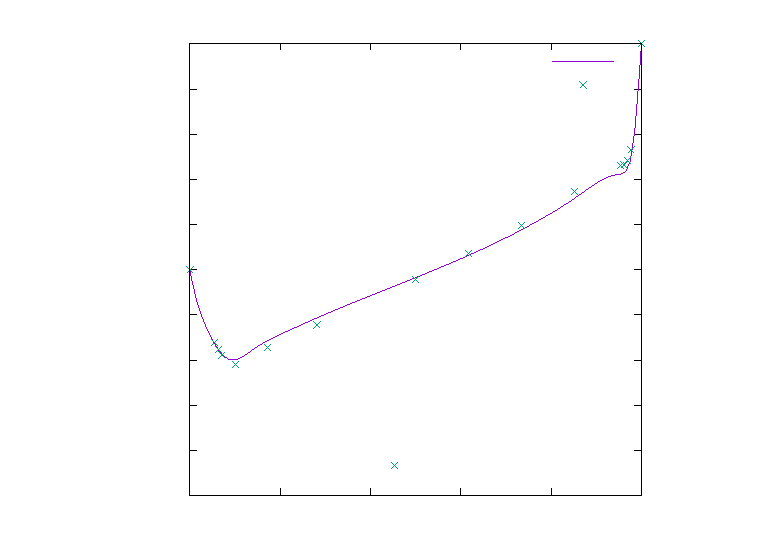
\includegraphics{u3200}}%
    \gplfronttext
  \end{picture}%
\endgroup
}
		\caption{$Re=3200$}
	\end{subfigure}
\end{figure}
\begin{figure}\ContinuedFloat
	\begin{subfigure}{0.5\textwidth}
		\resizebox{1.4\textwidth}{!}{% GNUPLOT: LaTeX picture with Postscript
\begingroup
  \makeatletter
  \providecommand\color[2][]{%
    \GenericError{(gnuplot) \space\space\space\@spaces}{%
      Package color not loaded in conjunction with
      terminal option `colourtext'%
    }{See the gnuplot documentation for explanation.%
    }{Either use 'blacktext' in gnuplot or load the package
      color.sty in LaTeX.}%
    \renewcommand\color[2][]{}%
  }%
  \providecommand\includegraphics[2][]{%
    \GenericError{(gnuplot) \space\space\space\@spaces}{%
      Package graphicx or graphics not loaded%
    }{See the gnuplot documentation for explanation.%
    }{The gnuplot epslatex terminal needs graphicx.sty or graphics.sty.}%
    \renewcommand\includegraphics[2][]{}%
  }%
  \providecommand\rotatebox[2]{#2}%
  \@ifundefined{ifGPcolor}{%
    \newif\ifGPcolor
    \GPcolortrue
  }{}%
  \@ifundefined{ifGPblacktext}{%
    \newif\ifGPblacktext
    \GPblacktexttrue
  }{}%
  % define a \g@addto@macro without @ in the name:
  \let\gplgaddtomacro\g@addto@macro
  % define empty templates for all commands taking text:
  \gdef\gplbacktext{}%
  \gdef\gplfronttext{}%
  \makeatother
  \ifGPblacktext
    % no textcolor at all
    \def\colorrgb#1{}%
    \def\colorgray#1{}%
  \else
    % gray or color?
    \ifGPcolor
      \def\colorrgb#1{\color[rgb]{#1}}%
      \def\colorgray#1{\color[gray]{#1}}%
      \expandafter\def\csname LTw\endcsname{\color{white}}%
      \expandafter\def\csname LTb\endcsname{\color{black}}%
      \expandafter\def\csname LTa\endcsname{\color{black}}%
      \expandafter\def\csname LT0\endcsname{\color[rgb]{1,0,0}}%
      \expandafter\def\csname LT1\endcsname{\color[rgb]{0,1,0}}%
      \expandafter\def\csname LT2\endcsname{\color[rgb]{0,0,1}}%
      \expandafter\def\csname LT3\endcsname{\color[rgb]{1,0,1}}%
      \expandafter\def\csname LT4\endcsname{\color[rgb]{0,1,1}}%
      \expandafter\def\csname LT5\endcsname{\color[rgb]{1,1,0}}%
      \expandafter\def\csname LT6\endcsname{\color[rgb]{0,0,0}}%
      \expandafter\def\csname LT7\endcsname{\color[rgb]{1,0.3,0}}%
      \expandafter\def\csname LT8\endcsname{\color[rgb]{0.5,0.5,0.5}}%
    \else
      % gray
      \def\colorrgb#1{\color{black}}%
      \def\colorgray#1{\color[gray]{#1}}%
      \expandafter\def\csname LTw\endcsname{\color{white}}%
      \expandafter\def\csname LTb\endcsname{\color{black}}%
      \expandafter\def\csname LTa\endcsname{\color{black}}%
      \expandafter\def\csname LT0\endcsname{\color{black}}%
      \expandafter\def\csname LT1\endcsname{\color{black}}%
      \expandafter\def\csname LT2\endcsname{\color{black}}%
      \expandafter\def\csname LT3\endcsname{\color{black}}%
      \expandafter\def\csname LT4\endcsname{\color{black}}%
      \expandafter\def\csname LT5\endcsname{\color{black}}%
      \expandafter\def\csname LT6\endcsname{\color{black}}%
      \expandafter\def\csname LT7\endcsname{\color{black}}%
      \expandafter\def\csname LT8\endcsname{\color{black}}%
    \fi
  \fi
    \setlength{\unitlength}{0.0500bp}%
    \ifx\gptboxheight\undefined%
      \newlength{\gptboxheight}%
      \newlength{\gptboxwidth}%
      \newsavebox{\gptboxtext}%
    \fi%
    \setlength{\fboxrule}{0.5pt}%
    \setlength{\fboxsep}{1pt}%
\begin{picture}(7200.00,5040.00)%
    \gplgaddtomacro\gplbacktext{%
      \csname LTb\endcsname%
      \put(1531,440){\makebox(0,0)[r]{\strut{}$-0.6$}}%
      \put(1531,982){\makebox(0,0)[r]{\strut{}$-0.4$}}%
      \put(1531,1524){\makebox(0,0)[r]{\strut{}$-0.2$}}%
      \put(1531,2066){\makebox(0,0)[r]{\strut{}$0$}}%
      \put(1531,2608){\makebox(0,0)[r]{\strut{}$0.2$}}%
      \put(1531,3149){\makebox(0,0)[r]{\strut{}$0.4$}}%
      \put(1531,3691){\makebox(0,0)[r]{\strut{}$0.6$}}%
      \put(1531,4233){\makebox(0,0)[r]{\strut{}$0.8$}}%
      \put(1531,4775){\makebox(0,0)[r]{\strut{}$1$}}%
      \put(1663,220){\makebox(0,0){\strut{}$0$}}%
      \put(2530,220){\makebox(0,0){\strut{}$0.2$}}%
      \put(3397,220){\makebox(0,0){\strut{}$0.4$}}%
      \put(4264,220){\makebox(0,0){\strut{}$0.6$}}%
      \put(5131,220){\makebox(0,0){\strut{}$0.8$}}%
      \put(5998,220){\makebox(0,0){\strut{}$1$}}%
    }%
    \gplgaddtomacro\gplfronttext{%
      \csname LTb\endcsname%
      \put(5011,4602){\makebox(0,0)[r]{\strut{}Calculated}}%
      \csname LTb\endcsname%
      \put(5011,4382){\makebox(0,0)[r]{\strut{}Reference}}%
    }%
    \gplbacktext
    \put(0,0){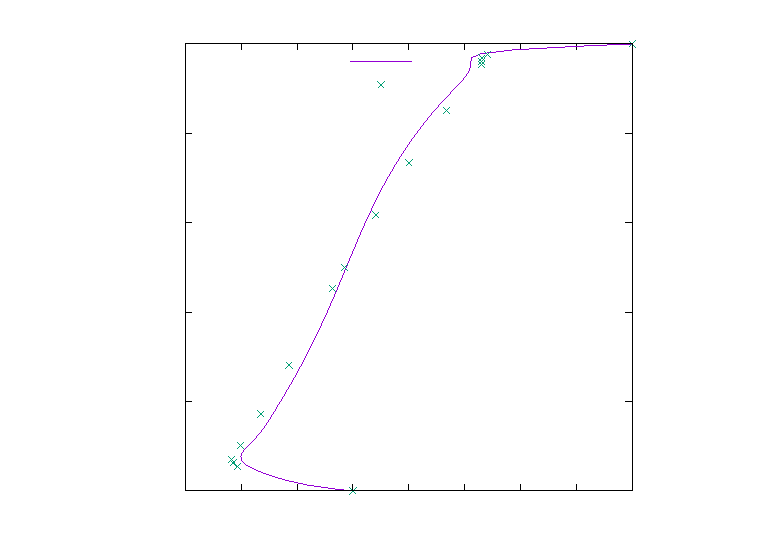
\includegraphics{DrivenCavity/u5000}}%
    \gplfronttext
  \end{picture}%
\endgroup
}
		\caption{$Re=5000$}
	\end{subfigure}%
	\begin{subfigure}{0.5\textwidth}
		\resizebox{1.4\textwidth}{!}{% GNUPLOT: LaTeX picture with Postscript
\begingroup
  \makeatletter
  \providecommand\color[2][]{%
    \GenericError{(gnuplot) \space\space\space\@spaces}{%
      Package color not loaded in conjunction with
      terminal option `colourtext'%
    }{See the gnuplot documentation for explanation.%
    }{Either use 'blacktext' in gnuplot or load the package
      color.sty in LaTeX.}%
    \renewcommand\color[2][]{}%
  }%
  \providecommand\includegraphics[2][]{%
    \GenericError{(gnuplot) \space\space\space\@spaces}{%
      Package graphicx or graphics not loaded%
    }{See the gnuplot documentation for explanation.%
    }{The gnuplot epslatex terminal needs graphicx.sty or graphics.sty.}%
    \renewcommand\includegraphics[2][]{}%
  }%
  \providecommand\rotatebox[2]{#2}%
  \@ifundefined{ifGPcolor}{%
    \newif\ifGPcolor
    \GPcolortrue
  }{}%
  \@ifundefined{ifGPblacktext}{%
    \newif\ifGPblacktext
    \GPblacktexttrue
  }{}%
  % define a \g@addto@macro without @ in the name:
  \let\gplgaddtomacro\g@addto@macro
  % define empty templates for all commands taking text:
  \gdef\gplbacktext{}%
  \gdef\gplfronttext{}%
  \makeatother
  \ifGPblacktext
    % no textcolor at all
    \def\colorrgb#1{}%
    \def\colorgray#1{}%
  \else
    % gray or color?
    \ifGPcolor
      \def\colorrgb#1{\color[rgb]{#1}}%
      \def\colorgray#1{\color[gray]{#1}}%
      \expandafter\def\csname LTw\endcsname{\color{white}}%
      \expandafter\def\csname LTb\endcsname{\color{black}}%
      \expandafter\def\csname LTa\endcsname{\color{black}}%
      \expandafter\def\csname LT0\endcsname{\color[rgb]{1,0,0}}%
      \expandafter\def\csname LT1\endcsname{\color[rgb]{0,1,0}}%
      \expandafter\def\csname LT2\endcsname{\color[rgb]{0,0,1}}%
      \expandafter\def\csname LT3\endcsname{\color[rgb]{1,0,1}}%
      \expandafter\def\csname LT4\endcsname{\color[rgb]{0,1,1}}%
      \expandafter\def\csname LT5\endcsname{\color[rgb]{1,1,0}}%
      \expandafter\def\csname LT6\endcsname{\color[rgb]{0,0,0}}%
      \expandafter\def\csname LT7\endcsname{\color[rgb]{1,0.3,0}}%
      \expandafter\def\csname LT8\endcsname{\color[rgb]{0.5,0.5,0.5}}%
    \else
      % gray
      \def\colorrgb#1{\color{black}}%
      \def\colorgray#1{\color[gray]{#1}}%
      \expandafter\def\csname LTw\endcsname{\color{white}}%
      \expandafter\def\csname LTb\endcsname{\color{black}}%
      \expandafter\def\csname LTa\endcsname{\color{black}}%
      \expandafter\def\csname LT0\endcsname{\color{black}}%
      \expandafter\def\csname LT1\endcsname{\color{black}}%
      \expandafter\def\csname LT2\endcsname{\color{black}}%
      \expandafter\def\csname LT3\endcsname{\color{black}}%
      \expandafter\def\csname LT4\endcsname{\color{black}}%
      \expandafter\def\csname LT5\endcsname{\color{black}}%
      \expandafter\def\csname LT6\endcsname{\color{black}}%
      \expandafter\def\csname LT7\endcsname{\color{black}}%
      \expandafter\def\csname LT8\endcsname{\color{black}}%
    \fi
  \fi
    \setlength{\unitlength}{0.0500bp}%
    \ifx\gptboxheight\undefined%
      \newlength{\gptboxheight}%
      \newlength{\gptboxwidth}%
      \newsavebox{\gptboxtext}%
    \fi%
    \setlength{\fboxrule}{0.5pt}%
    \setlength{\fboxsep}{1pt}%
\begin{picture}(7200.00,5040.00)%
    \gplgaddtomacro\gplbacktext{%
      \csname LTb\endcsname%
      \put(1531,440){\makebox(0,0)[r]{\strut{}$-0.6$}}%
      \put(1531,982){\makebox(0,0)[r]{\strut{}$-0.4$}}%
      \put(1531,1524){\makebox(0,0)[r]{\strut{}$-0.2$}}%
      \put(1531,2066){\makebox(0,0)[r]{\strut{}$0$}}%
      \put(1531,2608){\makebox(0,0)[r]{\strut{}$0.2$}}%
      \put(1531,3149){\makebox(0,0)[r]{\strut{}$0.4$}}%
      \put(1531,3691){\makebox(0,0)[r]{\strut{}$0.6$}}%
      \put(1531,4233){\makebox(0,0)[r]{\strut{}$0.8$}}%
      \put(1531,4775){\makebox(0,0)[r]{\strut{}$1$}}%
      \put(1663,220){\makebox(0,0){\strut{}$0$}}%
      \put(2530,220){\makebox(0,0){\strut{}$0.2$}}%
      \put(3397,220){\makebox(0,0){\strut{}$0.4$}}%
      \put(4264,220){\makebox(0,0){\strut{}$0.6$}}%
      \put(5131,220){\makebox(0,0){\strut{}$0.8$}}%
      \put(5998,220){\makebox(0,0){\strut{}$1$}}%
    }%
    \gplgaddtomacro\gplfronttext{%
      \csname LTb\endcsname%
      \put(5011,4602){\makebox(0,0)[r]{\strut{}Calculated}}%
      \csname LTb\endcsname%
      \put(5011,4382){\makebox(0,0)[r]{\strut{}Reference}}%
    }%
    \gplbacktext
    \put(0,0){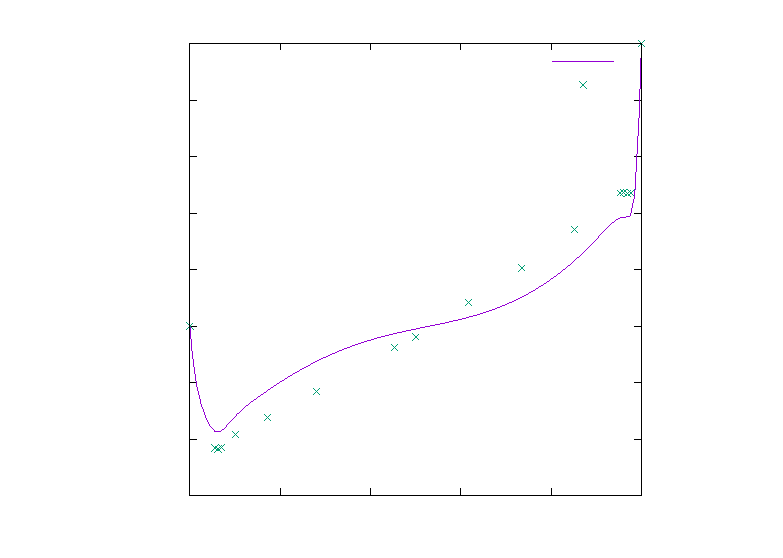
\includegraphics{DrivenCavity/u7500}}%
    \gplfronttext
  \end{picture}%
\endgroup
}
		\caption{$Re=7500$}
	\end{subfigure}
	\begin{subfigure}{0.5\textwidth}
		\center
		\resizebox{1.4\textwidth}{!}{% GNUPLOT: LaTeX picture with Postscript
\begingroup
  \makeatletter
  \providecommand\color[2][]{%
    \GenericError{(gnuplot) \space\space\space\@spaces}{%
      Package color not loaded in conjunction with
      terminal option `colourtext'%
    }{See the gnuplot documentation for explanation.%
    }{Either use 'blacktext' in gnuplot or load the package
      color.sty in LaTeX.}%
    \renewcommand\color[2][]{}%
  }%
  \providecommand\includegraphics[2][]{%
    \GenericError{(gnuplot) \space\space\space\@spaces}{%
      Package graphicx or graphics not loaded%
    }{See the gnuplot documentation for explanation.%
    }{The gnuplot epslatex terminal needs graphicx.sty or graphics.sty.}%
    \renewcommand\includegraphics[2][]{}%
  }%
  \providecommand\rotatebox[2]{#2}%
  \@ifundefined{ifGPcolor}{%
    \newif\ifGPcolor
    \GPcolortrue
  }{}%
  \@ifundefined{ifGPblacktext}{%
    \newif\ifGPblacktext
    \GPblacktexttrue
  }{}%
  % define a \g@addto@macro without @ in the name:
  \let\gplgaddtomacro\g@addto@macro
  % define empty templates for all commands taking text:
  \gdef\gplbacktext{}%
  \gdef\gplfronttext{}%
  \makeatother
  \ifGPblacktext
    % no textcolor at all
    \def\colorrgb#1{}%
    \def\colorgray#1{}%
  \else
    % gray or color?
    \ifGPcolor
      \def\colorrgb#1{\color[rgb]{#1}}%
      \def\colorgray#1{\color[gray]{#1}}%
      \expandafter\def\csname LTw\endcsname{\color{white}}%
      \expandafter\def\csname LTb\endcsname{\color{black}}%
      \expandafter\def\csname LTa\endcsname{\color{black}}%
      \expandafter\def\csname LT0\endcsname{\color[rgb]{1,0,0}}%
      \expandafter\def\csname LT1\endcsname{\color[rgb]{0,1,0}}%
      \expandafter\def\csname LT2\endcsname{\color[rgb]{0,0,1}}%
      \expandafter\def\csname LT3\endcsname{\color[rgb]{1,0,1}}%
      \expandafter\def\csname LT4\endcsname{\color[rgb]{0,1,1}}%
      \expandafter\def\csname LT5\endcsname{\color[rgb]{1,1,0}}%
      \expandafter\def\csname LT6\endcsname{\color[rgb]{0,0,0}}%
      \expandafter\def\csname LT7\endcsname{\color[rgb]{1,0.3,0}}%
      \expandafter\def\csname LT8\endcsname{\color[rgb]{0.5,0.5,0.5}}%
    \else
      % gray
      \def\colorrgb#1{\color{black}}%
      \def\colorgray#1{\color[gray]{#1}}%
      \expandafter\def\csname LTw\endcsname{\color{white}}%
      \expandafter\def\csname LTb\endcsname{\color{black}}%
      \expandafter\def\csname LTa\endcsname{\color{black}}%
      \expandafter\def\csname LT0\endcsname{\color{black}}%
      \expandafter\def\csname LT1\endcsname{\color{black}}%
      \expandafter\def\csname LT2\endcsname{\color{black}}%
      \expandafter\def\csname LT3\endcsname{\color{black}}%
      \expandafter\def\csname LT4\endcsname{\color{black}}%
      \expandafter\def\csname LT5\endcsname{\color{black}}%
      \expandafter\def\csname LT6\endcsname{\color{black}}%
      \expandafter\def\csname LT7\endcsname{\color{black}}%
      \expandafter\def\csname LT8\endcsname{\color{black}}%
    \fi
  \fi
    \setlength{\unitlength}{0.0500bp}%
    \ifx\gptboxheight\undefined%
      \newlength{\gptboxheight}%
      \newlength{\gptboxwidth}%
      \newsavebox{\gptboxtext}%
    \fi%
    \setlength{\fboxrule}{0.5pt}%
    \setlength{\fboxsep}{1pt}%
\begin{picture}(7200.00,5040.00)%
    \gplgaddtomacro\gplbacktext{%
      \csname LTb\endcsname%
      \put(1531,440){\makebox(0,0)[r]{\strut{}$-0.6$}}%
      \put(1531,982){\makebox(0,0)[r]{\strut{}$-0.4$}}%
      \put(1531,1524){\makebox(0,0)[r]{\strut{}$-0.2$}}%
      \put(1531,2066){\makebox(0,0)[r]{\strut{}$0$}}%
      \put(1531,2608){\makebox(0,0)[r]{\strut{}$0.2$}}%
      \put(1531,3149){\makebox(0,0)[r]{\strut{}$0.4$}}%
      \put(1531,3691){\makebox(0,0)[r]{\strut{}$0.6$}}%
      \put(1531,4233){\makebox(0,0)[r]{\strut{}$0.8$}}%
      \put(1531,4775){\makebox(0,0)[r]{\strut{}$1$}}%
      \put(1663,220){\makebox(0,0){\strut{}$0$}}%
      \put(2530,220){\makebox(0,0){\strut{}$0.2$}}%
      \put(3397,220){\makebox(0,0){\strut{}$0.4$}}%
      \put(4264,220){\makebox(0,0){\strut{}$0.6$}}%
      \put(5131,220){\makebox(0,0){\strut{}$0.8$}}%
      \put(5998,220){\makebox(0,0){\strut{}$1$}}%
    }%
    \gplgaddtomacro\gplfronttext{%
      \csname LTb\endcsname%
      \put(5011,4602){\makebox(0,0)[r]{\strut{}Calculated}}%
      \csname LTb\endcsname%
      \put(5011,4382){\makebox(0,0)[r]{\strut{}Reference}}%
    }%
    \gplbacktext
    \put(0,0){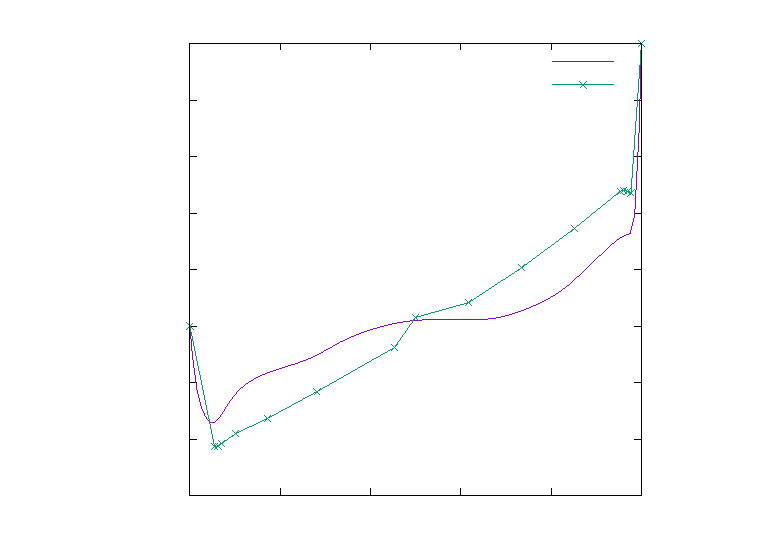
\includegraphics{u10000}}%
    \gplfronttext
  \end{picture}%
\endgroup
}
		\caption{$Re=10000$}
	\end{subfigure}
	\caption[Comparison between the reference solution and the calculated one of the horizontal velocity along the vertical line in the geometric center of the cavity]{Comparison between the reference solution and the calculated one of the horizontal velocity along the vertical line in the geometric center of the cavity \cite{Ghia1982}}
	\label{Drivenhorizontal}
\end{figure}

\begin{figure}[h]
	\centering
	\begin{subfigure}{0.5\textwidth}
		\resizebox{1.4\textwidth}{!}{% GNUPLOT: LaTeX picture with Postscript
\begingroup
  \makeatletter
  \providecommand\color[2][]{%
    \GenericError{(gnuplot) \space\space\space\@spaces}{%
      Package color not loaded in conjunction with
      terminal option `colourtext'%
    }{See the gnuplot documentation for explanation.%
    }{Either use 'blacktext' in gnuplot or load the package
      color.sty in LaTeX.}%
    \renewcommand\color[2][]{}%
  }%
  \providecommand\includegraphics[2][]{%
    \GenericError{(gnuplot) \space\space\space\@spaces}{%
      Package graphicx or graphics not loaded%
    }{See the gnuplot documentation for explanation.%
    }{The gnuplot epslatex terminal needs graphicx.sty or graphics.sty.}%
    \renewcommand\includegraphics[2][]{}%
  }%
  \providecommand\rotatebox[2]{#2}%
  \@ifundefined{ifGPcolor}{%
    \newif\ifGPcolor
    \GPcolortrue
  }{}%
  \@ifundefined{ifGPblacktext}{%
    \newif\ifGPblacktext
    \GPblacktexttrue
  }{}%
  % define a \g@addto@macro without @ in the name:
  \let\gplgaddtomacro\g@addto@macro
  % define empty templates for all commands taking text:
  \gdef\gplbacktext{}%
  \gdef\gplfronttext{}%
  \makeatother
  \ifGPblacktext
    % no textcolor at all
    \def\colorrgb#1{}%
    \def\colorgray#1{}%
  \else
    % gray or color?
    \ifGPcolor
      \def\colorrgb#1{\color[rgb]{#1}}%
      \def\colorgray#1{\color[gray]{#1}}%
      \expandafter\def\csname LTw\endcsname{\color{white}}%
      \expandafter\def\csname LTb\endcsname{\color{black}}%
      \expandafter\def\csname LTa\endcsname{\color{black}}%
      \expandafter\def\csname LT0\endcsname{\color[rgb]{1,0,0}}%
      \expandafter\def\csname LT1\endcsname{\color[rgb]{0,1,0}}%
      \expandafter\def\csname LT2\endcsname{\color[rgb]{0,0,1}}%
      \expandafter\def\csname LT3\endcsname{\color[rgb]{1,0,1}}%
      \expandafter\def\csname LT4\endcsname{\color[rgb]{0,1,1}}%
      \expandafter\def\csname LT5\endcsname{\color[rgb]{1,1,0}}%
      \expandafter\def\csname LT6\endcsname{\color[rgb]{0,0,0}}%
      \expandafter\def\csname LT7\endcsname{\color[rgb]{1,0.3,0}}%
      \expandafter\def\csname LT8\endcsname{\color[rgb]{0.5,0.5,0.5}}%
    \else
      % gray
      \def\colorrgb#1{\color{black}}%
      \def\colorgray#1{\color[gray]{#1}}%
      \expandafter\def\csname LTw\endcsname{\color{white}}%
      \expandafter\def\csname LTb\endcsname{\color{black}}%
      \expandafter\def\csname LTa\endcsname{\color{black}}%
      \expandafter\def\csname LT0\endcsname{\color{black}}%
      \expandafter\def\csname LT1\endcsname{\color{black}}%
      \expandafter\def\csname LT2\endcsname{\color{black}}%
      \expandafter\def\csname LT3\endcsname{\color{black}}%
      \expandafter\def\csname LT4\endcsname{\color{black}}%
      \expandafter\def\csname LT5\endcsname{\color{black}}%
      \expandafter\def\csname LT6\endcsname{\color{black}}%
      \expandafter\def\csname LT7\endcsname{\color{black}}%
      \expandafter\def\csname LT8\endcsname{\color{black}}%
    \fi
  \fi
    \setlength{\unitlength}{0.0500bp}%
    \ifx\gptboxheight\undefined%
      \newlength{\gptboxheight}%
      \newlength{\gptboxwidth}%
      \newsavebox{\gptboxtext}%
    \fi%
    \setlength{\fboxrule}{0.5pt}%
    \setlength{\fboxsep}{1pt}%
\begin{picture}(7200.00,5040.00)%
    \gplgaddtomacro\gplbacktext{%
      \csname LTb\endcsname%
      \put(1619,484){\makebox(0,0)[r]{\strut{}$-0.25$}}%
      \put(1619,961){\makebox(0,0)[r]{\strut{}$-0.2$}}%
      \put(1619,1438){\makebox(0,0)[r]{\strut{}$-0.15$}}%
      \put(1619,1914){\makebox(0,0)[r]{\strut{}$-0.1$}}%
      \put(1619,2391){\makebox(0,0)[r]{\strut{}$-0.05$}}%
      \put(1619,2868){\makebox(0,0)[r]{\strut{}$0$}}%
      \put(1619,3345){\makebox(0,0)[r]{\strut{}$0.05$}}%
      \put(1619,3821){\makebox(0,0)[r]{\strut{}$0.1$}}%
      \put(1619,4298){\makebox(0,0)[r]{\strut{}$0.15$}}%
      \put(1619,4775){\makebox(0,0)[r]{\strut{}$0.2$}}%
      \put(1751,264){\makebox(0,0){\strut{}$0$}}%
      \put(2609,264){\makebox(0,0){\strut{}$0.2$}}%
      \put(3467,264){\makebox(0,0){\strut{}$0.4$}}%
      \put(4326,264){\makebox(0,0){\strut{}$0.6$}}%
      \put(5184,264){\makebox(0,0){\strut{}$0.8$}}%
      \put(6042,264){\makebox(0,0){\strut{}$1$}}%
    }%
    \gplgaddtomacro\gplfronttext{%
      \csname LTb\endcsname%
      \put(1113,4829){\makebox(0,0){\strut{}v}}%
      \put(3896,154){\makebox(0,0){\strut{}x}}%
      \csname LTb\endcsname%
      \put(5055,4602){\makebox(0,0)[r]{\strut{}Calculated}}%
      \csname LTb\endcsname%
      \put(5055,4382){\makebox(0,0)[r]{\strut{}Reference}}%
    }%
    \gplbacktext
    \put(0,0){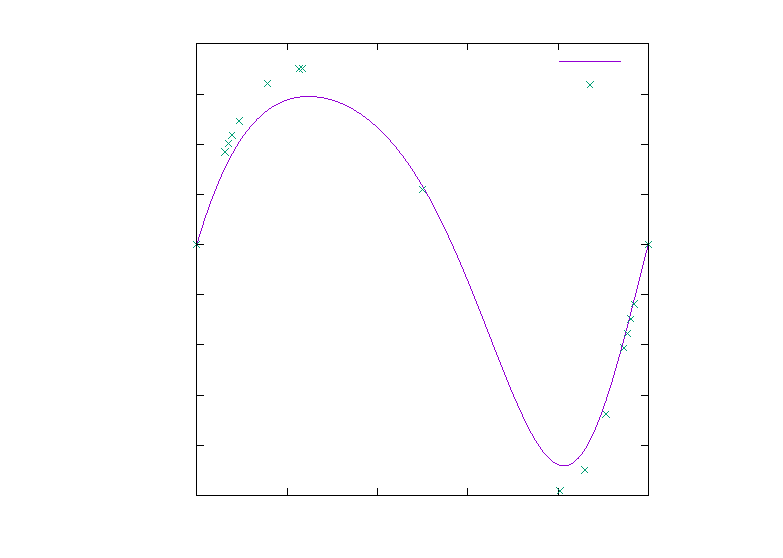
\includegraphics{DrivenCavity/v100}}%
    \gplfronttext
  \end{picture}%
\endgroup
}
		\caption{$Re=100$}
	\end{subfigure}%
	\begin{subfigure}{0.5\textwidth}
		\resizebox{1.4\textwidth}{!}{% GNUPLOT: LaTeX picture with Postscript
\begingroup
  \makeatletter
  \providecommand\color[2][]{%
    \GenericError{(gnuplot) \space\space\space\@spaces}{%
      Package color not loaded in conjunction with
      terminal option `colourtext'%
    }{See the gnuplot documentation for explanation.%
    }{Either use 'blacktext' in gnuplot or load the package
      color.sty in LaTeX.}%
    \renewcommand\color[2][]{}%
  }%
  \providecommand\includegraphics[2][]{%
    \GenericError{(gnuplot) \space\space\space\@spaces}{%
      Package graphicx or graphics not loaded%
    }{See the gnuplot documentation for explanation.%
    }{The gnuplot epslatex terminal needs graphicx.sty or graphics.sty.}%
    \renewcommand\includegraphics[2][]{}%
  }%
  \providecommand\rotatebox[2]{#2}%
  \@ifundefined{ifGPcolor}{%
    \newif\ifGPcolor
    \GPcolortrue
  }{}%
  \@ifundefined{ifGPblacktext}{%
    \newif\ifGPblacktext
    \GPblacktexttrue
  }{}%
  % define a \g@addto@macro without @ in the name:
  \let\gplgaddtomacro\g@addto@macro
  % define empty templates for all commands taking text:
  \gdef\gplbacktext{}%
  \gdef\gplfronttext{}%
  \makeatother
  \ifGPblacktext
    % no textcolor at all
    \def\colorrgb#1{}%
    \def\colorgray#1{}%
  \else
    % gray or color?
    \ifGPcolor
      \def\colorrgb#1{\color[rgb]{#1}}%
      \def\colorgray#1{\color[gray]{#1}}%
      \expandafter\def\csname LTw\endcsname{\color{white}}%
      \expandafter\def\csname LTb\endcsname{\color{black}}%
      \expandafter\def\csname LTa\endcsname{\color{black}}%
      \expandafter\def\csname LT0\endcsname{\color[rgb]{1,0,0}}%
      \expandafter\def\csname LT1\endcsname{\color[rgb]{0,1,0}}%
      \expandafter\def\csname LT2\endcsname{\color[rgb]{0,0,1}}%
      \expandafter\def\csname LT3\endcsname{\color[rgb]{1,0,1}}%
      \expandafter\def\csname LT4\endcsname{\color[rgb]{0,1,1}}%
      \expandafter\def\csname LT5\endcsname{\color[rgb]{1,1,0}}%
      \expandafter\def\csname LT6\endcsname{\color[rgb]{0,0,0}}%
      \expandafter\def\csname LT7\endcsname{\color[rgb]{1,0.3,0}}%
      \expandafter\def\csname LT8\endcsname{\color[rgb]{0.5,0.5,0.5}}%
    \else
      % gray
      \def\colorrgb#1{\color{black}}%
      \def\colorgray#1{\color[gray]{#1}}%
      \expandafter\def\csname LTw\endcsname{\color{white}}%
      \expandafter\def\csname LTb\endcsname{\color{black}}%
      \expandafter\def\csname LTa\endcsname{\color{black}}%
      \expandafter\def\csname LT0\endcsname{\color{black}}%
      \expandafter\def\csname LT1\endcsname{\color{black}}%
      \expandafter\def\csname LT2\endcsname{\color{black}}%
      \expandafter\def\csname LT3\endcsname{\color{black}}%
      \expandafter\def\csname LT4\endcsname{\color{black}}%
      \expandafter\def\csname LT5\endcsname{\color{black}}%
      \expandafter\def\csname LT6\endcsname{\color{black}}%
      \expandafter\def\csname LT7\endcsname{\color{black}}%
      \expandafter\def\csname LT8\endcsname{\color{black}}%
    \fi
  \fi
    \setlength{\unitlength}{0.0500bp}%
    \ifx\gptboxheight\undefined%
      \newlength{\gptboxheight}%
      \newlength{\gptboxwidth}%
      \newsavebox{\gptboxtext}%
    \fi%
    \setlength{\fboxrule}{0.5pt}%
    \setlength{\fboxsep}{1pt}%
\begin{picture}(7200.00,5040.00)%
    \gplgaddtomacro\gplbacktext{%
      \csname LTb\endcsname%
      \put(1531,440){\makebox(0,0)[r]{\strut{}$-0.5$}}%
      \put(1531,922){\makebox(0,0)[r]{\strut{}$-0.4$}}%
      \put(1531,1403){\makebox(0,0)[r]{\strut{}$-0.3$}}%
      \put(1531,1885){\makebox(0,0)[r]{\strut{}$-0.2$}}%
      \put(1531,2367){\makebox(0,0)[r]{\strut{}$-0.1$}}%
      \put(1531,2848){\makebox(0,0)[r]{\strut{}$0$}}%
      \put(1531,3330){\makebox(0,0)[r]{\strut{}$0.1$}}%
      \put(1531,3812){\makebox(0,0)[r]{\strut{}$0.2$}}%
      \put(1531,4293){\makebox(0,0)[r]{\strut{}$0.3$}}%
      \put(1531,4775){\makebox(0,0)[r]{\strut{}$0.4$}}%
      \put(1663,220){\makebox(0,0){\strut{}$0$}}%
      \put(2530,220){\makebox(0,0){\strut{}$0.2$}}%
      \put(3397,220){\makebox(0,0){\strut{}$0.4$}}%
      \put(4264,220){\makebox(0,0){\strut{}$0.6$}}%
      \put(5131,220){\makebox(0,0){\strut{}$0.8$}}%
      \put(5998,220){\makebox(0,0){\strut{}$1$}}%
    }%
    \gplgaddtomacro\gplfronttext{%
      \csname LTb\endcsname%
      \put(5011,4602){\makebox(0,0)[r]{\strut{}Calculated}}%
      \csname LTb\endcsname%
      \put(5011,4382){\makebox(0,0)[r]{\strut{}Reference}}%
    }%
    \gplbacktext
    \put(0,0){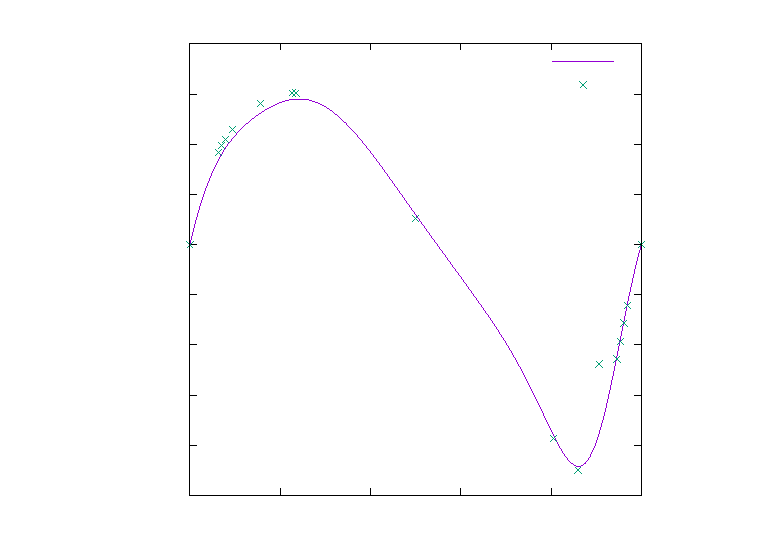
\includegraphics{DrivenCavity/v400}}%
    \gplfronttext
  \end{picture}%
\endgroup
}
		\caption{$Re=400$}
	\end{subfigure}
	\begin{subfigure}{0.5\textwidth}
		\resizebox{1.4\textwidth}{!}{% GNUPLOT: LaTeX picture with Postscript
\begingroup
  \makeatletter
  \providecommand\color[2][]{%
    \GenericError{(gnuplot) \space\space\space\@spaces}{%
      Package color not loaded in conjunction with
      terminal option `colourtext'%
    }{See the gnuplot documentation for explanation.%
    }{Either use 'blacktext' in gnuplot or load the package
      color.sty in LaTeX.}%
    \renewcommand\color[2][]{}%
  }%
  \providecommand\includegraphics[2][]{%
    \GenericError{(gnuplot) \space\space\space\@spaces}{%
      Package graphicx or graphics not loaded%
    }{See the gnuplot documentation for explanation.%
    }{The gnuplot epslatex terminal needs graphicx.sty or graphics.sty.}%
    \renewcommand\includegraphics[2][]{}%
  }%
  \providecommand\rotatebox[2]{#2}%
  \@ifundefined{ifGPcolor}{%
    \newif\ifGPcolor
    \GPcolortrue
  }{}%
  \@ifundefined{ifGPblacktext}{%
    \newif\ifGPblacktext
    \GPblacktexttrue
  }{}%
  % define a \g@addto@macro without @ in the name:
  \let\gplgaddtomacro\g@addto@macro
  % define empty templates for all commands taking text:
  \gdef\gplbacktext{}%
  \gdef\gplfronttext{}%
  \makeatother
  \ifGPblacktext
    % no textcolor at all
    \def\colorrgb#1{}%
    \def\colorgray#1{}%
  \else
    % gray or color?
    \ifGPcolor
      \def\colorrgb#1{\color[rgb]{#1}}%
      \def\colorgray#1{\color[gray]{#1}}%
      \expandafter\def\csname LTw\endcsname{\color{white}}%
      \expandafter\def\csname LTb\endcsname{\color{black}}%
      \expandafter\def\csname LTa\endcsname{\color{black}}%
      \expandafter\def\csname LT0\endcsname{\color[rgb]{1,0,0}}%
      \expandafter\def\csname LT1\endcsname{\color[rgb]{0,1,0}}%
      \expandafter\def\csname LT2\endcsname{\color[rgb]{0,0,1}}%
      \expandafter\def\csname LT3\endcsname{\color[rgb]{1,0,1}}%
      \expandafter\def\csname LT4\endcsname{\color[rgb]{0,1,1}}%
      \expandafter\def\csname LT5\endcsname{\color[rgb]{1,1,0}}%
      \expandafter\def\csname LT6\endcsname{\color[rgb]{0,0,0}}%
      \expandafter\def\csname LT7\endcsname{\color[rgb]{1,0.3,0}}%
      \expandafter\def\csname LT8\endcsname{\color[rgb]{0.5,0.5,0.5}}%
    \else
      % gray
      \def\colorrgb#1{\color{black}}%
      \def\colorgray#1{\color[gray]{#1}}%
      \expandafter\def\csname LTw\endcsname{\color{white}}%
      \expandafter\def\csname LTb\endcsname{\color{black}}%
      \expandafter\def\csname LTa\endcsname{\color{black}}%
      \expandafter\def\csname LT0\endcsname{\color{black}}%
      \expandafter\def\csname LT1\endcsname{\color{black}}%
      \expandafter\def\csname LT2\endcsname{\color{black}}%
      \expandafter\def\csname LT3\endcsname{\color{black}}%
      \expandafter\def\csname LT4\endcsname{\color{black}}%
      \expandafter\def\csname LT5\endcsname{\color{black}}%
      \expandafter\def\csname LT6\endcsname{\color{black}}%
      \expandafter\def\csname LT7\endcsname{\color{black}}%
      \expandafter\def\csname LT8\endcsname{\color{black}}%
    \fi
  \fi
    \setlength{\unitlength}{0.0500bp}%
    \ifx\gptboxheight\undefined%
      \newlength{\gptboxheight}%
      \newlength{\gptboxwidth}%
      \newsavebox{\gptboxtext}%
    \fi%
    \setlength{\fboxrule}{0.5pt}%
    \setlength{\fboxsep}{1pt}%
\begin{picture}(7200.00,5040.00)%
    \gplgaddtomacro\gplbacktext{%
      \csname LTb\endcsname%
      \put(1531,440){\makebox(0,0)[r]{\strut{}$-0.6$}}%
      \put(1531,873){\makebox(0,0)[r]{\strut{}$-0.5$}}%
      \put(1531,1307){\makebox(0,0)[r]{\strut{}$-0.4$}}%
      \put(1531,1740){\makebox(0,0)[r]{\strut{}$-0.3$}}%
      \put(1531,2174){\makebox(0,0)[r]{\strut{}$-0.2$}}%
      \put(1531,2607){\makebox(0,0)[r]{\strut{}$-0.1$}}%
      \put(1531,3041){\makebox(0,0)[r]{\strut{}$0$}}%
      \put(1531,3475){\makebox(0,0)[r]{\strut{}$0.1$}}%
      \put(1531,3908){\makebox(0,0)[r]{\strut{}$0.2$}}%
      \put(1531,4342){\makebox(0,0)[r]{\strut{}$0.3$}}%
      \put(1531,4775){\makebox(0,0)[r]{\strut{}$0.4$}}%
      \put(1663,220){\makebox(0,0){\strut{}$0$}}%
      \put(2530,220){\makebox(0,0){\strut{}$0.2$}}%
      \put(3397,220){\makebox(0,0){\strut{}$0.4$}}%
      \put(4264,220){\makebox(0,0){\strut{}$0.6$}}%
      \put(5131,220){\makebox(0,0){\strut{}$0.8$}}%
      \put(5998,220){\makebox(0,0){\strut{}$1$}}%
    }%
    \gplgaddtomacro\gplfronttext{%
      \csname LTb\endcsname%
      \put(5011,4602){\makebox(0,0)[r]{\strut{}Calculated}}%
      \csname LTb\endcsname%
      \put(5011,4382){\makebox(0,0)[r]{\strut{}Reference}}%
    }%
    \gplbacktext
    \put(0,0){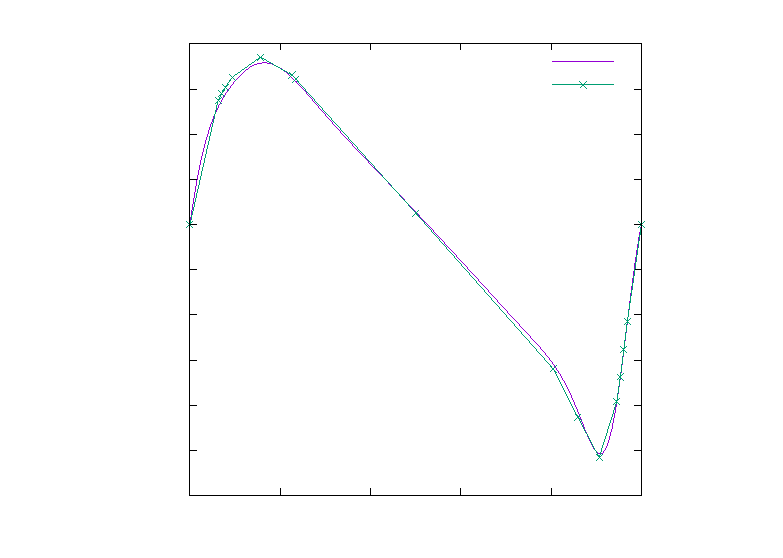
\includegraphics{v1000}}%
    \gplfronttext
  \end{picture}%
\endgroup
}
		\caption{$Re=1000$}
	\end{subfigure}%
	\begin{subfigure}{0.5\textwidth}
		\resizebox{1.4\textwidth}{!}{% GNUPLOT: LaTeX picture with Postscript
\begingroup
  \makeatletter
  \providecommand\color[2][]{%
    \GenericError{(gnuplot) \space\space\space\@spaces}{%
      Package color not loaded in conjunction with
      terminal option `colourtext'%
    }{See the gnuplot documentation for explanation.%
    }{Either use 'blacktext' in gnuplot or load the package
      color.sty in LaTeX.}%
    \renewcommand\color[2][]{}%
  }%
  \providecommand\includegraphics[2][]{%
    \GenericError{(gnuplot) \space\space\space\@spaces}{%
      Package graphicx or graphics not loaded%
    }{See the gnuplot documentation for explanation.%
    }{The gnuplot epslatex terminal needs graphicx.sty or graphics.sty.}%
    \renewcommand\includegraphics[2][]{}%
  }%
  \providecommand\rotatebox[2]{#2}%
  \@ifundefined{ifGPcolor}{%
    \newif\ifGPcolor
    \GPcolortrue
  }{}%
  \@ifundefined{ifGPblacktext}{%
    \newif\ifGPblacktext
    \GPblacktexttrue
  }{}%
  % define a \g@addto@macro without @ in the name:
  \let\gplgaddtomacro\g@addto@macro
  % define empty templates for all commands taking text:
  \gdef\gplbacktext{}%
  \gdef\gplfronttext{}%
  \makeatother
  \ifGPblacktext
    % no textcolor at all
    \def\colorrgb#1{}%
    \def\colorgray#1{}%
  \else
    % gray or color?
    \ifGPcolor
      \def\colorrgb#1{\color[rgb]{#1}}%
      \def\colorgray#1{\color[gray]{#1}}%
      \expandafter\def\csname LTw\endcsname{\color{white}}%
      \expandafter\def\csname LTb\endcsname{\color{black}}%
      \expandafter\def\csname LTa\endcsname{\color{black}}%
      \expandafter\def\csname LT0\endcsname{\color[rgb]{1,0,0}}%
      \expandafter\def\csname LT1\endcsname{\color[rgb]{0,1,0}}%
      \expandafter\def\csname LT2\endcsname{\color[rgb]{0,0,1}}%
      \expandafter\def\csname LT3\endcsname{\color[rgb]{1,0,1}}%
      \expandafter\def\csname LT4\endcsname{\color[rgb]{0,1,1}}%
      \expandafter\def\csname LT5\endcsname{\color[rgb]{1,1,0}}%
      \expandafter\def\csname LT6\endcsname{\color[rgb]{0,0,0}}%
      \expandafter\def\csname LT7\endcsname{\color[rgb]{1,0.3,0}}%
      \expandafter\def\csname LT8\endcsname{\color[rgb]{0.5,0.5,0.5}}%
    \else
      % gray
      \def\colorrgb#1{\color{black}}%
      \def\colorgray#1{\color[gray]{#1}}%
      \expandafter\def\csname LTw\endcsname{\color{white}}%
      \expandafter\def\csname LTb\endcsname{\color{black}}%
      \expandafter\def\csname LTa\endcsname{\color{black}}%
      \expandafter\def\csname LT0\endcsname{\color{black}}%
      \expandafter\def\csname LT1\endcsname{\color{black}}%
      \expandafter\def\csname LT2\endcsname{\color{black}}%
      \expandafter\def\csname LT3\endcsname{\color{black}}%
      \expandafter\def\csname LT4\endcsname{\color{black}}%
      \expandafter\def\csname LT5\endcsname{\color{black}}%
      \expandafter\def\csname LT6\endcsname{\color{black}}%
      \expandafter\def\csname LT7\endcsname{\color{black}}%
      \expandafter\def\csname LT8\endcsname{\color{black}}%
    \fi
  \fi
    \setlength{\unitlength}{0.0500bp}%
    \ifx\gptboxheight\undefined%
      \newlength{\gptboxheight}%
      \newlength{\gptboxwidth}%
      \newsavebox{\gptboxtext}%
    \fi%
    \setlength{\fboxrule}{0.5pt}%
    \setlength{\fboxsep}{1pt}%
\begin{picture}(7200.00,5040.00)%
    \gplgaddtomacro\gplbacktext{%
      \csname LTb\endcsname%
      \put(1531,440){\makebox(0,0)[r]{\strut{}$-0.6$}}%
      \put(1531,834){\makebox(0,0)[r]{\strut{}$-0.5$}}%
      \put(1531,1228){\makebox(0,0)[r]{\strut{}$-0.4$}}%
      \put(1531,1622){\makebox(0,0)[r]{\strut{}$-0.3$}}%
      \put(1531,2016){\makebox(0,0)[r]{\strut{}$-0.2$}}%
      \put(1531,2410){\makebox(0,0)[r]{\strut{}$-0.1$}}%
      \put(1531,2805){\makebox(0,0)[r]{\strut{}$0$}}%
      \put(1531,3199){\makebox(0,0)[r]{\strut{}$0.1$}}%
      \put(1531,3593){\makebox(0,0)[r]{\strut{}$0.2$}}%
      \put(1531,3987){\makebox(0,0)[r]{\strut{}$0.3$}}%
      \put(1531,4381){\makebox(0,0)[r]{\strut{}$0.4$}}%
      \put(1531,4775){\makebox(0,0)[r]{\strut{}$0.5$}}%
      \put(1663,220){\makebox(0,0){\strut{}$0$}}%
      \put(2530,220){\makebox(0,0){\strut{}$0.2$}}%
      \put(3397,220){\makebox(0,0){\strut{}$0.4$}}%
      \put(4264,220){\makebox(0,0){\strut{}$0.6$}}%
      \put(5131,220){\makebox(0,0){\strut{}$0.8$}}%
      \put(5998,220){\makebox(0,0){\strut{}$1$}}%
    }%
    \gplgaddtomacro\gplfronttext{%
      \csname LTb\endcsname%
      \put(5011,4602){\makebox(0,0)[r]{\strut{}Calculated}}%
      \csname LTb\endcsname%
      \put(5011,4382){\makebox(0,0)[r]{\strut{}Reference}}%
    }%
    \gplbacktext
    \put(0,0){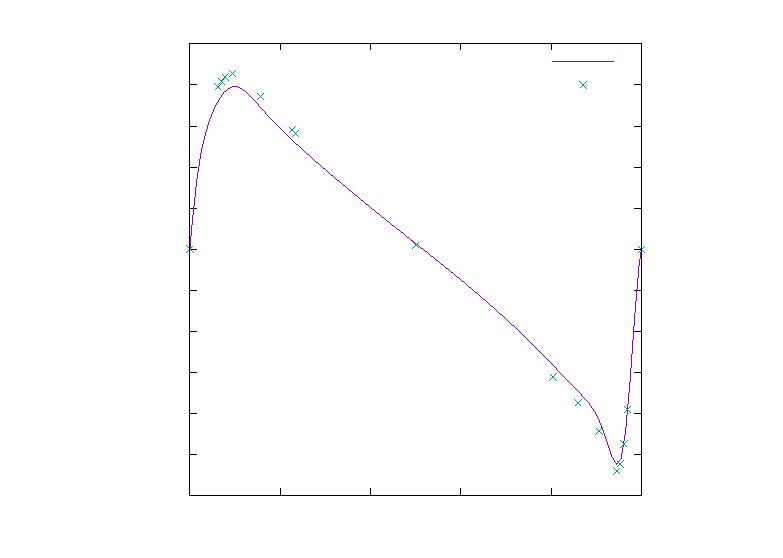
\includegraphics{DrivenCavity/v3200}}%
    \gplfronttext
  \end{picture}%
\endgroup
}
		\caption{$Re=3200$}
	\end{subfigure}
\end{figure}
\begin{figure}\ContinuedFloat
	\begin{subfigure}{0.5\textwidth}
		\resizebox{1.4\textwidth}{!}{% GNUPLOT: LaTeX picture with Postscript
\begingroup
  \makeatletter
  \providecommand\color[2][]{%
    \GenericError{(gnuplot) \space\space\space\@spaces}{%
      Package color not loaded in conjunction with
      terminal option `colourtext'%
    }{See the gnuplot documentation for explanation.%
    }{Either use 'blacktext' in gnuplot or load the package
      color.sty in LaTeX.}%
    \renewcommand\color[2][]{}%
  }%
  \providecommand\includegraphics[2][]{%
    \GenericError{(gnuplot) \space\space\space\@spaces}{%
      Package graphicx or graphics not loaded%
    }{See the gnuplot documentation for explanation.%
    }{The gnuplot epslatex terminal needs graphicx.sty or graphics.sty.}%
    \renewcommand\includegraphics[2][]{}%
  }%
  \providecommand\rotatebox[2]{#2}%
  \@ifundefined{ifGPcolor}{%
    \newif\ifGPcolor
    \GPcolortrue
  }{}%
  \@ifundefined{ifGPblacktext}{%
    \newif\ifGPblacktext
    \GPblacktexttrue
  }{}%
  % define a \g@addto@macro without @ in the name:
  \let\gplgaddtomacro\g@addto@macro
  % define empty templates for all commands taking text:
  \gdef\gplbacktext{}%
  \gdef\gplfronttext{}%
  \makeatother
  \ifGPblacktext
    % no textcolor at all
    \def\colorrgb#1{}%
    \def\colorgray#1{}%
  \else
    % gray or color?
    \ifGPcolor
      \def\colorrgb#1{\color[rgb]{#1}}%
      \def\colorgray#1{\color[gray]{#1}}%
      \expandafter\def\csname LTw\endcsname{\color{white}}%
      \expandafter\def\csname LTb\endcsname{\color{black}}%
      \expandafter\def\csname LTa\endcsname{\color{black}}%
      \expandafter\def\csname LT0\endcsname{\color[rgb]{1,0,0}}%
      \expandafter\def\csname LT1\endcsname{\color[rgb]{0,1,0}}%
      \expandafter\def\csname LT2\endcsname{\color[rgb]{0,0,1}}%
      \expandafter\def\csname LT3\endcsname{\color[rgb]{1,0,1}}%
      \expandafter\def\csname LT4\endcsname{\color[rgb]{0,1,1}}%
      \expandafter\def\csname LT5\endcsname{\color[rgb]{1,1,0}}%
      \expandafter\def\csname LT6\endcsname{\color[rgb]{0,0,0}}%
      \expandafter\def\csname LT7\endcsname{\color[rgb]{1,0.3,0}}%
      \expandafter\def\csname LT8\endcsname{\color[rgb]{0.5,0.5,0.5}}%
    \else
      % gray
      \def\colorrgb#1{\color{black}}%
      \def\colorgray#1{\color[gray]{#1}}%
      \expandafter\def\csname LTw\endcsname{\color{white}}%
      \expandafter\def\csname LTb\endcsname{\color{black}}%
      \expandafter\def\csname LTa\endcsname{\color{black}}%
      \expandafter\def\csname LT0\endcsname{\color{black}}%
      \expandafter\def\csname LT1\endcsname{\color{black}}%
      \expandafter\def\csname LT2\endcsname{\color{black}}%
      \expandafter\def\csname LT3\endcsname{\color{black}}%
      \expandafter\def\csname LT4\endcsname{\color{black}}%
      \expandafter\def\csname LT5\endcsname{\color{black}}%
      \expandafter\def\csname LT6\endcsname{\color{black}}%
      \expandafter\def\csname LT7\endcsname{\color{black}}%
      \expandafter\def\csname LT8\endcsname{\color{black}}%
    \fi
  \fi
    \setlength{\unitlength}{0.0500bp}%
    \ifx\gptboxheight\undefined%
      \newlength{\gptboxheight}%
      \newlength{\gptboxwidth}%
      \newsavebox{\gptboxtext}%
    \fi%
    \setlength{\fboxrule}{0.5pt}%
    \setlength{\fboxsep}{1pt}%
\begin{picture}(7200.00,5040.00)%
    \gplgaddtomacro\gplbacktext{%
      \csname LTb\endcsname%
      \put(1553,484){\makebox(0,0)[r]{\strut{}$-0.6$}}%
      \put(1553,874){\makebox(0,0)[r]{\strut{}$-0.5$}}%
      \put(1553,1264){\makebox(0,0)[r]{\strut{}$-0.4$}}%
      \put(1553,1654){\makebox(0,0)[r]{\strut{}$-0.3$}}%
      \put(1553,2044){\makebox(0,0)[r]{\strut{}$-0.2$}}%
      \put(1553,2434){\makebox(0,0)[r]{\strut{}$-0.1$}}%
      \put(1553,2825){\makebox(0,0)[r]{\strut{}$0$}}%
      \put(1553,3215){\makebox(0,0)[r]{\strut{}$0.1$}}%
      \put(1553,3605){\makebox(0,0)[r]{\strut{}$0.2$}}%
      \put(1553,3995){\makebox(0,0)[r]{\strut{}$0.3$}}%
      \put(1553,4385){\makebox(0,0)[r]{\strut{}$0.4$}}%
      \put(1553,4775){\makebox(0,0)[r]{\strut{}$0.5$}}%
      \put(1685,264){\makebox(0,0){\strut{}$0$}}%
      \put(2543,264){\makebox(0,0){\strut{}$0.2$}}%
      \put(3401,264){\makebox(0,0){\strut{}$0.4$}}%
      \put(4260,264){\makebox(0,0){\strut{}$0.6$}}%
      \put(5118,264){\makebox(0,0){\strut{}$0.8$}}%
      \put(5976,264){\makebox(0,0){\strut{}$1$}}%
    }%
    \gplgaddtomacro\gplfronttext{%
      \csname LTb\endcsname%
      \put(1179,4829){\makebox(0,0){\strut{}v}}%
      \put(3830,154){\makebox(0,0){\strut{}x}}%
      \csname LTb\endcsname%
      \put(4989,4602){\makebox(0,0)[r]{\strut{}Calculated}}%
      \csname LTb\endcsname%
      \put(4989,4382){\makebox(0,0)[r]{\strut{}Reference}}%
    }%
    \gplbacktext
    \put(0,0){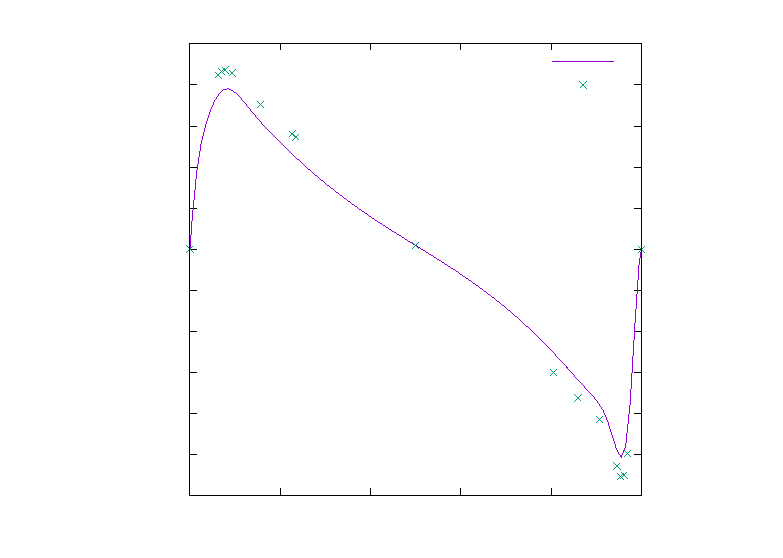
\includegraphics{DrivenCavity/v5000}}%
    \gplfronttext
  \end{picture}%
\endgroup
}
		\caption{$Re=5000$}
	\end{subfigure}%
	\begin{subfigure}{0.5\textwidth}
		\resizebox{1.4\textwidth}{!}{% GNUPLOT: LaTeX picture with Postscript
\begingroup
  \makeatletter
  \providecommand\color[2][]{%
    \GenericError{(gnuplot) \space\space\space\@spaces}{%
      Package color not loaded in conjunction with
      terminal option `colourtext'%
    }{See the gnuplot documentation for explanation.%
    }{Either use 'blacktext' in gnuplot or load the package
      color.sty in LaTeX.}%
    \renewcommand\color[2][]{}%
  }%
  \providecommand\includegraphics[2][]{%
    \GenericError{(gnuplot) \space\space\space\@spaces}{%
      Package graphicx or graphics not loaded%
    }{See the gnuplot documentation for explanation.%
    }{The gnuplot epslatex terminal needs graphicx.sty or graphics.sty.}%
    \renewcommand\includegraphics[2][]{}%
  }%
  \providecommand\rotatebox[2]{#2}%
  \@ifundefined{ifGPcolor}{%
    \newif\ifGPcolor
    \GPcolortrue
  }{}%
  \@ifundefined{ifGPblacktext}{%
    \newif\ifGPblacktext
    \GPblacktexttrue
  }{}%
  % define a \g@addto@macro without @ in the name:
  \let\gplgaddtomacro\g@addto@macro
  % define empty templates for all commands taking text:
  \gdef\gplbacktext{}%
  \gdef\gplfronttext{}%
  \makeatother
  \ifGPblacktext
    % no textcolor at all
    \def\colorrgb#1{}%
    \def\colorgray#1{}%
  \else
    % gray or color?
    \ifGPcolor
      \def\colorrgb#1{\color[rgb]{#1}}%
      \def\colorgray#1{\color[gray]{#1}}%
      \expandafter\def\csname LTw\endcsname{\color{white}}%
      \expandafter\def\csname LTb\endcsname{\color{black}}%
      \expandafter\def\csname LTa\endcsname{\color{black}}%
      \expandafter\def\csname LT0\endcsname{\color[rgb]{1,0,0}}%
      \expandafter\def\csname LT1\endcsname{\color[rgb]{0,1,0}}%
      \expandafter\def\csname LT2\endcsname{\color[rgb]{0,0,1}}%
      \expandafter\def\csname LT3\endcsname{\color[rgb]{1,0,1}}%
      \expandafter\def\csname LT4\endcsname{\color[rgb]{0,1,1}}%
      \expandafter\def\csname LT5\endcsname{\color[rgb]{1,1,0}}%
      \expandafter\def\csname LT6\endcsname{\color[rgb]{0,0,0}}%
      \expandafter\def\csname LT7\endcsname{\color[rgb]{1,0.3,0}}%
      \expandafter\def\csname LT8\endcsname{\color[rgb]{0.5,0.5,0.5}}%
    \else
      % gray
      \def\colorrgb#1{\color{black}}%
      \def\colorgray#1{\color[gray]{#1}}%
      \expandafter\def\csname LTw\endcsname{\color{white}}%
      \expandafter\def\csname LTb\endcsname{\color{black}}%
      \expandafter\def\csname LTa\endcsname{\color{black}}%
      \expandafter\def\csname LT0\endcsname{\color{black}}%
      \expandafter\def\csname LT1\endcsname{\color{black}}%
      \expandafter\def\csname LT2\endcsname{\color{black}}%
      \expandafter\def\csname LT3\endcsname{\color{black}}%
      \expandafter\def\csname LT4\endcsname{\color{black}}%
      \expandafter\def\csname LT5\endcsname{\color{black}}%
      \expandafter\def\csname LT6\endcsname{\color{black}}%
      \expandafter\def\csname LT7\endcsname{\color{black}}%
      \expandafter\def\csname LT8\endcsname{\color{black}}%
    \fi
  \fi
    \setlength{\unitlength}{0.0500bp}%
    \ifx\gptboxheight\undefined%
      \newlength{\gptboxheight}%
      \newlength{\gptboxwidth}%
      \newsavebox{\gptboxtext}%
    \fi%
    \setlength{\fboxrule}{0.5pt}%
    \setlength{\fboxsep}{1pt}%
\begin{picture}(7200.00,5040.00)%
    \gplgaddtomacro\gplbacktext{%
      \csname LTb\endcsname%
      \put(1553,484){\makebox(0,0)[r]{\strut{}$-0.6$}}%
      \put(1553,874){\makebox(0,0)[r]{\strut{}$-0.5$}}%
      \put(1553,1264){\makebox(0,0)[r]{\strut{}$-0.4$}}%
      \put(1553,1654){\makebox(0,0)[r]{\strut{}$-0.3$}}%
      \put(1553,2044){\makebox(0,0)[r]{\strut{}$-0.2$}}%
      \put(1553,2434){\makebox(0,0)[r]{\strut{}$-0.1$}}%
      \put(1553,2825){\makebox(0,0)[r]{\strut{}$0$}}%
      \put(1553,3215){\makebox(0,0)[r]{\strut{}$0.1$}}%
      \put(1553,3605){\makebox(0,0)[r]{\strut{}$0.2$}}%
      \put(1553,3995){\makebox(0,0)[r]{\strut{}$0.3$}}%
      \put(1553,4385){\makebox(0,0)[r]{\strut{}$0.4$}}%
      \put(1553,4775){\makebox(0,0)[r]{\strut{}$0.5$}}%
      \put(1685,264){\makebox(0,0){\strut{}$0$}}%
      \put(2543,264){\makebox(0,0){\strut{}$0.2$}}%
      \put(3401,264){\makebox(0,0){\strut{}$0.4$}}%
      \put(4260,264){\makebox(0,0){\strut{}$0.6$}}%
      \put(5118,264){\makebox(0,0){\strut{}$0.8$}}%
      \put(5976,264){\makebox(0,0){\strut{}$1$}}%
    }%
    \gplgaddtomacro\gplfronttext{%
      \csname LTb\endcsname%
      \put(1179,4829){\makebox(0,0){\strut{}v}}%
      \put(3830,154){\makebox(0,0){\strut{}x}}%
      \csname LTb\endcsname%
      \put(4989,4602){\makebox(0,0)[r]{\strut{}Calculated}}%
      \csname LTb\endcsname%
      \put(4989,4382){\makebox(0,0)[r]{\strut{}Reference}}%
    }%
    \gplbacktext
    \put(0,0){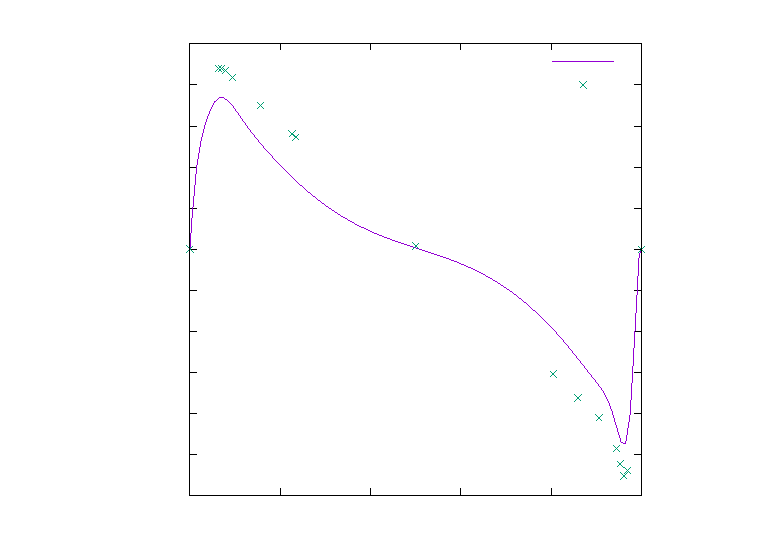
\includegraphics{DrivenCavity/v7500}}%
    \gplfronttext
  \end{picture}%
\endgroup
}
		\caption{$Re=7500$}
	\end{subfigure}
	\begin{subfigure}{0.5\textwidth}
		\center
		\resizebox{1.4\textwidth}{!}{% GNUPLOT: LaTeX picture with Postscript
\begingroup
  \makeatletter
  \providecommand\color[2][]{%
    \GenericError{(gnuplot) \space\space\space\@spaces}{%
      Package color not loaded in conjunction with
      terminal option `colourtext'%
    }{See the gnuplot documentation for explanation.%
    }{Either use 'blacktext' in gnuplot or load the package
      color.sty in LaTeX.}%
    \renewcommand\color[2][]{}%
  }%
  \providecommand\includegraphics[2][]{%
    \GenericError{(gnuplot) \space\space\space\@spaces}{%
      Package graphicx or graphics not loaded%
    }{See the gnuplot documentation for explanation.%
    }{The gnuplot epslatex terminal needs graphicx.sty or graphics.sty.}%
    \renewcommand\includegraphics[2][]{}%
  }%
  \providecommand\rotatebox[2]{#2}%
  \@ifundefined{ifGPcolor}{%
    \newif\ifGPcolor
    \GPcolortrue
  }{}%
  \@ifundefined{ifGPblacktext}{%
    \newif\ifGPblacktext
    \GPblacktexttrue
  }{}%
  % define a \g@addto@macro without @ in the name:
  \let\gplgaddtomacro\g@addto@macro
  % define empty templates for all commands taking text:
  \gdef\gplbacktext{}%
  \gdef\gplfronttext{}%
  \makeatother
  \ifGPblacktext
    % no textcolor at all
    \def\colorrgb#1{}%
    \def\colorgray#1{}%
  \else
    % gray or color?
    \ifGPcolor
      \def\colorrgb#1{\color[rgb]{#1}}%
      \def\colorgray#1{\color[gray]{#1}}%
      \expandafter\def\csname LTw\endcsname{\color{white}}%
      \expandafter\def\csname LTb\endcsname{\color{black}}%
      \expandafter\def\csname LTa\endcsname{\color{black}}%
      \expandafter\def\csname LT0\endcsname{\color[rgb]{1,0,0}}%
      \expandafter\def\csname LT1\endcsname{\color[rgb]{0,1,0}}%
      \expandafter\def\csname LT2\endcsname{\color[rgb]{0,0,1}}%
      \expandafter\def\csname LT3\endcsname{\color[rgb]{1,0,1}}%
      \expandafter\def\csname LT4\endcsname{\color[rgb]{0,1,1}}%
      \expandafter\def\csname LT5\endcsname{\color[rgb]{1,1,0}}%
      \expandafter\def\csname LT6\endcsname{\color[rgb]{0,0,0}}%
      \expandafter\def\csname LT7\endcsname{\color[rgb]{1,0.3,0}}%
      \expandafter\def\csname LT8\endcsname{\color[rgb]{0.5,0.5,0.5}}%
    \else
      % gray
      \def\colorrgb#1{\color{black}}%
      \def\colorgray#1{\color[gray]{#1}}%
      \expandafter\def\csname LTw\endcsname{\color{white}}%
      \expandafter\def\csname LTb\endcsname{\color{black}}%
      \expandafter\def\csname LTa\endcsname{\color{black}}%
      \expandafter\def\csname LT0\endcsname{\color{black}}%
      \expandafter\def\csname LT1\endcsname{\color{black}}%
      \expandafter\def\csname LT2\endcsname{\color{black}}%
      \expandafter\def\csname LT3\endcsname{\color{black}}%
      \expandafter\def\csname LT4\endcsname{\color{black}}%
      \expandafter\def\csname LT5\endcsname{\color{black}}%
      \expandafter\def\csname LT6\endcsname{\color{black}}%
      \expandafter\def\csname LT7\endcsname{\color{black}}%
      \expandafter\def\csname LT8\endcsname{\color{black}}%
    \fi
  \fi
    \setlength{\unitlength}{0.0500bp}%
    \ifx\gptboxheight\undefined%
      \newlength{\gptboxheight}%
      \newlength{\gptboxwidth}%
      \newsavebox{\gptboxtext}%
    \fi%
    \setlength{\fboxrule}{0.5pt}%
    \setlength{\fboxsep}{1pt}%
\begin{picture}(7200.00,5040.00)%
    \gplgaddtomacro\gplbacktext{%
      \csname LTb\endcsname%
      \put(1531,440){\makebox(0,0)[r]{\strut{}$-0.6$}}%
      \put(1531,834){\makebox(0,0)[r]{\strut{}$-0.5$}}%
      \put(1531,1228){\makebox(0,0)[r]{\strut{}$-0.4$}}%
      \put(1531,1622){\makebox(0,0)[r]{\strut{}$-0.3$}}%
      \put(1531,2016){\makebox(0,0)[r]{\strut{}$-0.2$}}%
      \put(1531,2410){\makebox(0,0)[r]{\strut{}$-0.1$}}%
      \put(1531,2805){\makebox(0,0)[r]{\strut{}$0$}}%
      \put(1531,3199){\makebox(0,0)[r]{\strut{}$0.1$}}%
      \put(1531,3593){\makebox(0,0)[r]{\strut{}$0.2$}}%
      \put(1531,3987){\makebox(0,0)[r]{\strut{}$0.3$}}%
      \put(1531,4381){\makebox(0,0)[r]{\strut{}$0.4$}}%
      \put(1531,4775){\makebox(0,0)[r]{\strut{}$0.5$}}%
      \put(1663,220){\makebox(0,0){\strut{}$0$}}%
      \put(2530,220){\makebox(0,0){\strut{}$0.2$}}%
      \put(3397,220){\makebox(0,0){\strut{}$0.4$}}%
      \put(4264,220){\makebox(0,0){\strut{}$0.6$}}%
      \put(5131,220){\makebox(0,0){\strut{}$0.8$}}%
      \put(5998,220){\makebox(0,0){\strut{}$1$}}%
    }%
    \gplgaddtomacro\gplfronttext{%
      \csname LTb\endcsname%
      \put(5011,4602){\makebox(0,0)[r]{\strut{}Calculated}}%
      \csname LTb\endcsname%
      \put(5011,4382){\makebox(0,0)[r]{\strut{}Reference}}%
    }%
    \gplbacktext
    \put(0,0){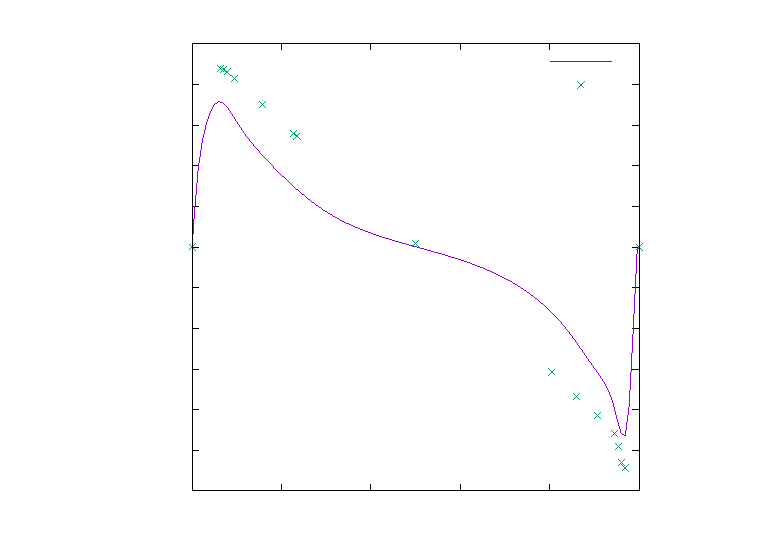
\includegraphics{DrivenCavity/v10000}}%
    \gplfronttext
  \end{picture}%
\endgroup
}
		\caption{$Re=10000$}
	\end{subfigure}
	\caption[Comparison between the reference solution and the calculated one of the vertical velocity along the horizontal line in the geometric center of the cavity]{Comparison between the reference solution and the calculated one of the vertical velocity along the horizontal line in the geometric center of the cavity \cite{Ghia1982}}
	\label{Drivenvertical}
\end{figure}